\documentclass{article}
\usepackage[round]{natbib}
\usepackage{amsmath,amssymb,amsfonts}%
\usepackage{geometry}%
\usepackage{color}
\usepackage{graphicx}
\usepackage{authblk}
\usepackage{nameref}
\usepackage[right]{lineno}
\usepackage{subcaption}
\usepackage{tikz}
\usetikzlibrary{calc,positioning}
\usepackage{url}
% JK: turning this off for the moment as I keep clicking through on links
% to the bibliography while reading the text and it's intensely annoying.
% Can reinstate when we're ready to preprint
% \usepackage[hidelinks]{hyperref}

\newcommand{\noderef}[1]{\textsf{#1}}
\newcommand{\tsinfer}[0]{\texttt{tsinfer}}
\newcommand{\kwarg}[0]{\texttt{KwARG}}
\newcommand{\argweaver}[0]{\texttt{ARGweaver}}
\newcommand{\relate}[0]{\texttt{Relate}}
\newcommand{\espalier}[0]{\texttt{Espalier}}

\begin{document}

\linenumbers
\title{A general and efficient representation of Ancestral Recombination Graphs}

% First authors
\author[1]{Yan Wong}

% Second authors
\author[2,$\star$]{Anastasia Ignatieva}
\author[3,$\star$]{Jere Koskela}

% Middle Authors
\author[4]{Gregor Gorjanc}
\author[5]{Anthony W. Wohns}

% Corresponding
\author[1,$\dagger$]{Jerome Kelleher}

\affil[1]{Big Data Institute, Li Ka Shing Centre for Health Information and Discovery, University of Oxford, OX3 7LF, UK}
\affil[2]{Department of Statistics, University of Oxford, OX1 3LB, UK}
\affil[3]{Department of Statistics, University of Warwick, CV4 7AL, UK}
\affil[4]{The Roslin Institute and Royal (Dick) School of Veterinary Studies, University of Edinburgh, EH25 9RG, UK}
\affil[5]{Broad Institute of MIT and Harvard, Cambridge, MA 02142, USA}

\affil[$\star$]{Denotes shared second authorship, listed alphabetically}
\affil[$\dagger$]{Denotes corresponding author}


\maketitle

% FIXME this is weak, but gives the basic outline
\begin{abstract}
Recent breakthroughs have made it possible to infer genetic genealogies in
the presence of recombination at scale, enabling many
downstream applications in population and statistical genetics.
The structure representing such recombinant genetic ancestry
is usually referred to as an Ancestral Recombination Graph (ARG),
although there is some confusion about the interpretation and little
agreement on the concrete details.
We propose a concrete definition of ARGs
in terms of genomes and their intervals of genetic inheritance (gARG)
and contrast this with the classical event-based definition (eARG).
The eARG definition is based on the coalescent with recombination
stochastic process, and we show how the assumptions of that process
place limitations on the patterns of inheritance that can be
represented, and that these assumptions are
% Better wording
substantially broken
in modern large-scale datasets.
Representing genetic ancestry
with an eARG also requires complete precision about the ordering
of all recombination events, which we will rarely have sufficient
information to infer.
We show, in contrast, that the gARG definition
can fully capture the richness of modern large-scale datasets,
enables fine-grained
levels of precision about recombination to be represented,
and forms the basis of an efficient computational framework.
\end{abstract}

\textbf{Keywords:} Ancestral recombination graphs

\section*{Introduction}
% Inferring the genetic relationships between sampled genomes in the form of a
% phylogenetic tree is a necessary prerequisite for many analyses of
% species~\citep{rannala2003genetics}, non-recombining sections of
% DNA~\citep{cann1987mitochondrial,underhill2001annalsofhumangenetics}
% and viruses~\citep{grenfell2004science}.
% A phylogenetic tree captures information about the genealogy
% of the sample in an elegant and concise
% way, by postulating a set of ancestors common to the samples
% together with paths of inheritance between them. A rich literature exists
% on analysing the mathematical properties of these
% trees~\citep{steel2016phylogeny}, and numerous
% methods exist to infer them~\citep{felsenstein2004inferring}.
% However, the genetic genealogy of a recombining organism
% cannot be captured by a single tree: instead,
% the inheritance of each section of the genome may be described
% by a (slightly) different local tree~\citep{hudson1983properties}.
% Inferring complex
% genealogies of this nature
% presents profound technical difficulties, meaning genealogy-based approaches have
% not been widely used in population and statistical genetics.
% Until recently, analysis of
% population genetic data has therefore primarily focussed on summaries derived
% from the local trees~\citep{tajima1983evolutionary,tavare1984line}
% rather than using the full underlying genealogy itself. Such
% derived measures include allele frequencies and site frequency
% spectra~\citep{achaz2009frequency,ralph2020efficiently},
% patterns of linkage disequilibrium~\citep{mcvean2002genealogical}, and
% principal components~\citep{mcvean2009genealogical}.
Estimating the detailed genetic genealogy of a set of sequences
under the influence of recombination,
usually known as an Ancestral Recombination Graph (ARG), is a long-standing
goal in genetics.
Recent breakthroughs
in large-scale inference
methods~\citep{rasmussen2014genome,kelleher2019inferring,speidel2019method,
schaefer2021ancestral,wohns2022unified,zhang2023biobank,zhan2023towards}
and data representation~\citep{kelleher2016efficient,kelleher2018efficient}
have raised the realistic prospect of ARG-based analysis becoming a standard part
of the population and statistical genetics toolkit~\citep{hejase2020summary}.
Applications using these inferred ancestries as inputs have begun to
appear~\citep{osmond2021estimating,fan2022genealogical,hejase2022deep,zhang2023biobank,
% TODO update when natgen paper comes out
nowbandegani2022extremely}
and many more are sure to
follow~\citep{harris2019database,harris2023using}.

% TODO need to mention ARG-as-a-data-structure to clarify.
% What is the problem?
Although it is widely accepted that ARGs are important, there is significant
confusion about what, precisely, an ARG \emph{is}. [THIS IS BAD, WHY?]
We also lack a shared format for interchanging ARG data [which is bad
for users, progress]. [Because we don't really agree on what an ARG is,
we don't really know what properties it should have, when we infer it].

% What do we do?
Here we precisely define an encoding for ARGs based on specific genomes
and their intervals of genetic inheritance. We contrast this ``gARG''
encoding with the classical approach derived from the coalescent
with recombination stochastic process of Griffiths
and colleagues~\citep{griffiths1991two,ethier1990two,
griffiths1996ancestral,griffiths1997ancestral}. As this is based
on recording evolutionary events, we refer to it as the event ARG, or
``eARG'' encoding.
We show that the gARG encoding is both flexible and efficient,
and can represent varying levels of precision about historical
events.
[MORE]

% and because it is focused on encoding the \emph{outcome}
% of evolutionary events rather than the details of the events themselves,

% In this paper we [turn into proper round up paragraph later]
% \begin{enumerate}
% \item Discuss the classical Ancestral Recombination Graph formulation,
% and show how it derives from (and is limited by) the coalescent with
% recombination.
% \item In the following sections we
% show that, although the ARG-as-a-data-structure perspective is
% now the most common interpretation, the \emph{form} of that
% data structure is still closely linked to the original
% stochastic process, and that this form is inflexible
% in the types of genetic inheritance that can be described,
% computationally inefficient, and
% forces complete (and potentially spurious) precision about
% the location and timing
% of recombination events. % (and coalescent events?)
% \item Suggest a definition of ARGs that is free of these limitations,
% where the formulation is derived from a (normally diploid) pedigree rather than from
% coalescent approximations, and where the genetic
% material which is transmitted is described by annotations attached to
% edges rather than nodes.
% \item Suggest a classification of ARG nodes that helps us to understand
% the properties of the structures inferred by different methods, and illustrate
% with some examples.

% \item This, coupled with
%     the explicit association of genome coordinates with edges, allows
%     us to represent even the bewilderingly complex patterns of relatedness
%     present in modern datasets.

% \end{enumerate}


% \section*{Genome ARGs}\label{eARG}
% In keeping with its original derivation in terms of a stochastic
% process (see Appendix~\ref{sec-arg-history}), the classical definition of an
% ARG data structure is
% in terms of events.
% Nodes represent
% common ancestor or recombination events that occurred in the
% history of some set of sample genomes, and edges represent ancestral
% lineages~\citep{griffiths1996ancestral}.
% In a common ancestor event the inbound lineages are merged into a
% single ancestral lineage, and in a recombination
% event a lineage is split into two independent
% ancestral lineages.
% % The final vital
% % detail is that we associate a breakpoint with each recombination
% % event.
% % This information is sufficient to uniquely
% % define the local genealogical trees at every position along the genome,
% % which is the basic requirement for a data structure encoding
% % genome-wide genetic ancestry.
% As illustrated in Fig.~\ref{fig-arg-data-structure}, this information
% is usually concretely encoded by associating a recombination breakpoint
% (which is null for common ancestor events) and an ordered list of parents
% with each node. We refer to such a  data structure as an
% ``event ARG'' (eARG).
% To recover the local tree at genome coordinate $x$ (the most
% fundamental operation required for an ARG data structure),
% we traverse the graph rootwards from the leaves.
% At a particular
% node $u$, if it has one parent we are at a common ancestor
% node and we follow that parent. If we are at a
% recombination node, $u$ has two parents: if
% $x$ is less than the breakpoint we follow
% the edge to the first parent, and otherwise follow the edge
% to the second parent.
% The order in which parents are listed at a recombination node is
% therefore significant, telling us
% from which parent the segments of genome to the left and right of the breakpoint
% were inherited.

% This ordering requirement, while straightforward
% to describe, has some practical drawbacks. For example,
% % Surely the meaning is clear from the context here and we don't need
% % qualify the meaning of ``ARG''
% when using this representation and simulating an ARG backwards in time,
% the first event older than a recombination may involve the lineage carrying the
% ancestry to the right of the breakpoint rather
% than the left, and so we cannot emit edges as they are generated.
% Such issues can be worked around, of course, but depending on the ordering of
% otherwise indistinguishable objects is generally problematic.

% \begin{figure}
% \centering
% % \begin{tabular}{cc}
% \begin{tikzpicture}[x=5mm, y=5mm, node distance=2mm and 20mm]
% \tikzset{greynode/.style={circle,fill,inner sep=1},
% nodelabel/.style={font=\footnotesize}}

% \node (s0) [greynode] at (0, 0) {};
% \node (s1) [greynode] at (3, 0) {};
% \node (s2) [greynode] at (6, 0) {};
% \node (s3) [greynode] at (3, 1) {};
% \node (s4) [greynode] at (1, 2) {};
% \node (s5) [greynode] at (5, 3) {};
% \node (s6) [greynode] at (3, 4) {};

% % \node [anchor=north west] at (0,6) {A};
% \node [nodelabel,anchor=north west] at ($(s3) + (0,0)$) {$x$};
% \foreach \u/\lab in {s0/$\textsf{a}$, s1/$\textsf{b}$, s2/$\textsf{c}$} \node[nodelabel,anchor=north] at (\u) {\lab};
% \foreach \u/\lab in {s4/$\textsf{e}$} \node[nodelabel,anchor=south west] at (\u) {\lab};
% \foreach \u/\lab in {s5/$\textsf{f}$} \node[nodelabel,anchor=south east] at (\u) {\lab};
% \foreach \u/\lab in {s3/$\textsf{d}$, s6/$\textsf{g}$} \node[nodelabel,anchor=south] at (\u) {\lab};

% %% Edges
% \draw (s1) -- (s3);
% \draw (s0) |- (s4);
% \draw (s4) -- (2,2) |- (s3);
% \draw (s4) |- (s6);
% \draw (s3) -- (4,1) |- (s5);
% \draw (s2) |- (s5);
% \draw (s5) |- (s6);

% % \node [anchor=north west] at (9,6) {B};
% \node [nodelabel,anchor=north west] at ($(10,5)$) {
% \begin{tabular}{c|c|l}
% % \multicolumn{2}{c}{Breakpoints}\\
% Node & Breakpoint & Parents\\
% \hline
% $\noderef{a}$ & $\varnothing$ & [\noderef{e}]\\
% $\noderef{b}$ & $\varnothing$ & [\noderef{d}] \\
% $\noderef{c}$ & $\varnothing$ & [\noderef{f}]\\
% $\noderef{d}$ & $x$ & [\noderef{e}, \noderef{f}] \\
% $\noderef{e}$ & $\varnothing$ & [\noderef{g}]\\
% $\noderef{f}$ & $\varnothing$ & [\noderef{g}]\\
% $\noderef{g}$ & $\varnothing$ & []\\
% \end{tabular}};


% % \node [anchor=north west] at (9,6) {C};
% % \node [nodelabel,anchor=north west] at ($(10,5)$) {
% % \begin{tabular}{ll}
% % Edges & Intervals\\
% % \hline
% % $(\textsf{a}, \textsf{e})$ & $(0, L]$ \\
% % $(\textsf{b}, \textsf{d})$ & $(0, L]$ \\
% % $(\textsf{c}, \textsf{f})$ & $(0, L]$ \\
% % $(\textsf{d}, \textsf{e})$ & $(0, x]$ \\
% % $(\textsf{d}, \textsf{f})$ & $(x, L]$ \\
% % $(\textsf{e}, \textsf{g})$ & $(0, L]$ \\
% % $(\textsf{f}, \textsf{g})$ & $(0, L]$ \\
% % \end{tabular}};


% \end{tikzpicture}
% \caption{\label{fig-arg-data-structure}
% A graphical depiction of a classical event ARG and a concrete
% encoding of the information. Node \noderef{d} is a recombination
% event as it is associated with a non-null breakpoint, and has
% two parents. Nodes \noderef{e}, \noderef{f} and \noderef{g} are
% common ancestor events.
% }
% \end{figure}

% % What do we mean by an eARG, formally?
% To be concrete, we can formally define the
% classical Griffiths eARG as a tuple $(e, \sigma)$, where $e$
% is an ordered list of edges defining a directed acyclic graph and
% $\sigma: \mathbb{N} \rightarrow \mathbb{N}$
% is a function mapping nodes to recombination breakpoints,
% such that $\sigma(u) = x$
% if $u$ is a recombination event with breakpoint $x$ and
% $\sigma(u) = \varnothing$ otherwise.
% (This is equivalent to having different ``types''
% of node, where breakpoints are associated with recombination
% nodes only).
% Each edge $e_j = (c, p)$ describes an edge between
% child node $c$ and parent $p$, where $c, p \in \mathbb{N}$.
% % For each recombination node $u$ we must
% % have exactly two edges in $e$ such that $u$ is the child.
% This encoding of an eARG is equivalent to the output
% of programs such as
% \texttt{ARGweaver}~\citep{rasmussen2014genome}
% and \texttt{KwARG}~\citep{ignatieva2021kwarg},
% and an example is given in Fig.~\ref{fig-arg-data-structure}A.
% Note that the description above captures only the
% graph topology: if we also wish to know the branch lengths we need
% an additional function $t(u): \mathbb{N} \rightarrow \mathbb{R}$
% which defines the time of each node.

% In practice,
% several methods explicitly associate information with the outbound edges
% of a recombination event
% to resolve the issue~\citep{lyngso2005minimum,ignatieva2021kwarg}.

% TODO update this when later sections have been drafted.
% As we see in sections XXX and YYY there are substantial limitations
% of expressivity and computational performance when using this eARG
% encoding. More fundamentally, however, the general approach
% of classifying nodes according to a discrete set of events
% and associating genome information with those nodes is intrinsically
% limiting. As we saw in the previous section, the original ARG
% definitions were derived directly from the coalescent with recombination
% stochastic process, and the types of ancestry that can be
% described are therefore limited by the assumptions of that
% model.

% JK: Removing stuff about the limitations of the encoding here
% because it's reasonably straightforward to see an extension in
% which the number of breakpoints is in less than the number of
% parents, and it starts muddying the waters a bit.

% The eARG encoding consists of two types of event
% (common ancestor and recombination) but nature is not so parsimonious
% and there are many other processes that will affect the
% ancestry of samples.
% For example, gene conversion between homologous
% chromosomes~\citep{wiuf2000coalescent,chen2007gene} is an important
% evolutionary force in many species~\cite[e.g.][]{yang2012great}.
% % Some refs for where people are inferring ancestry in the
% % presence of GC? Isn't this what ClonalFrame etc are all about?
% Similarly, the eARG encoding cannot easily represent multiple
% recombinations on a chromosome, or the transmission of multiple
% chromosomes.
% What we can infer about ancestral histories and
% processes should not be limited by the data structure that we
% use to represent such ancestry. The eARG is simply one way
% to \emph{encode} such history, and, as we have shown,
% one that has significant limitations of expressivity
% derived from its historical origins in the idealised model of
% coalescent with recombination.

% \section*{Node vs edge annotations}
% Another aspect of the classical description of an ARG data structure that
% derives from its historical origins as a stochastic
% process is how we encode information about genetic
% inheritance in the graph. The approach taken by Griffiths to
% doing this is elegant: all we need to do is store
% the location of the breakpoint at each recombination event.
% % Storing a breakpoint for each recombinatin event is a very
% % natural and straightforward thing to do when simulating
% % an  ARG process.
% Given the graph topology and these breakpoints, we can then
% recover the
% local trees at every point in the genome
% by tracing rootwards from the leaves and choosing the
% appropriate outbound path at recombination nodes.
% However, there are several significant disadvantages
% to this approach: [TODO be concrete here later
% and give pointers to the section where we discuss the
% alternative.]

% Fortunately, there is a straightforward change to the
% classical eARG encoding that simplifies
% implementations and greatly increases the flexibility
% of both the types and granularity of inheritance information
% that we can represent.
% The main change that we need to make is to associate
% the details of inheritance with \emph{edges} rather than
% as breakpoints associated with recombination events and
% edge ordering rules.
% This is illustrated in Fig~\ref{fig-arg-data-structure}C
% where this alternative edge annotation formulation is
% shown. By associating the interval $(0, x)$ with edge $(d,e)$
% and the interval $(x, L)$ with $(d, f)$ we make the encoding
% unambiguous: we can list the edges in any order, and it
% will describe the same set of local genealogical trees.
% This approach is also more flexible, because any pattern
% of inheritance can be described by these intervals. For
% example, if a gene conversion event occurred where a segment
% between positions $x$ and $y$ was inherited by
% node $d$ from $e$, we would state this by associating
% the intervals $\{(0, x], (y, L]\}$ with $(d,e)$ and
% $\{(x, y]\}$ with $(d,f)$.
% This change is straightforward, involves no loss of information
% and (as we see in later sections)
% greatly increases both the expressivity and computational
% power of ancestral recombination graph data structures.

\section*{Genome ARGs}
% There is no fundamental reason, however, that the data structure we use
% to describe patterns of genetic inheritance must be in terms
% of specific causal events. As demonstrated in subsequent sections,
% there are significant advantages to using
% a slightly different formulation, which
% we call a ``genome ARG'' (gARG).
In this section we define a concrete definition of an ARG in terms
of particular genomes and their patterns of inheritance, which
we refer to as a ``genome ARG``, or gARG.
First, let us define a genome as the complete set of genetic material that a child
inherits from one parent (i.e., haploids have one genome, diploids two, etc.).
Then, a gARG is a graph in which nodes represent
monoploid genomes  and edges represent
genetic inheritance between an ancestor and a descendant,
where each edge is annotated with the coordinates
of the genomic intervals over which genetic inheritance occurs.
We can therefore view a gARG for a given set of individuals
as a subset of their pedigree, but, crucially,
where each individual is represented by two nodes (for diploids).
% To recover the local tree for a genomic
% position $x$, we traverse the graph rootwards from the leaves
% (as in an eARG) and at a particular node, we follow the outbound
% edge associated with the genomic interval containing $x$.
% Recent discussions have illustrated the
% relationship between ARGs and
% pedigrees~\citep{mathieson2020ancestry,brandt2021evaluation},
% and the deep connections between the structures are
% well understood
% \citep[e.g.][]{wakeley2012genetics,gusfield2014recombinatorics,
% speed2015naturereviewsgenetics}.
This is illustrated in Fig.~\ref{fig-arg-in-pedigree},
which
shows how the genomes embedded in an example (highly inbred)
pedigree correspond to the nodes in a gARG.
In this diploid example
a genome is inherited from one
of the individual's parents,
and may be the recombined product of that parent's two genomes.
For example, individual $I_1$ in Fig.~\ref{fig-arg-in-pedigree}
has two genomes \textsf{a} and \textsf{b},
inherited from parents $I_3$ and $I_4$. Genome \textsf{a} is the product of
recombining $I_3$'s two genomes \textsf{e} and \textsf{f} at position 2,
whereas \textsf{b} was inherited directly from $I_4$'s genome \textsf{g} without
recombination.

\begin{figure}
\begin{center}
    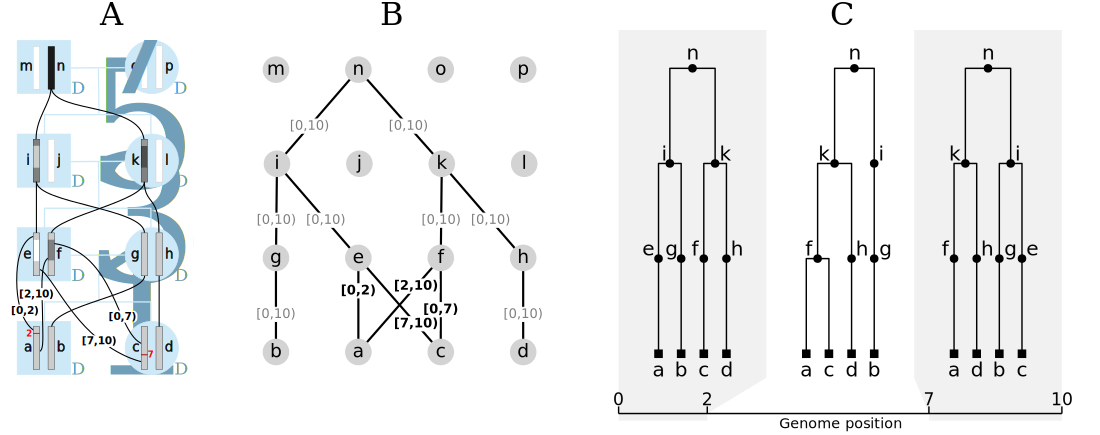
\includegraphics[width=\textwidth]{illustrations/arg-in-pedigree}
\end{center}
\caption{\label{fig-arg-in-pedigree}
% TODO caption needs another pass. One the full section has been written
% it'll be clearer what we need to say in the caption vs the text.
An example gARG embedded in a pedigree.
(A) Diploid individuals, visualised in a highly inbred pedigree and
labelled $I_1$ to $I_8$, contain both paternal  and maternal  genomes
labelled \textsf{a} to \textsf{p}. Black lines show inheritance paths connecting
genomes in the current generation (\textsf{a} to \textsf{d}) with their ancestors.
Genomes \textsf{a} and \textsf{c} are independent recombinants of
the paternal genomes \textsf{e}
% Gregor: there is some overlap between a and c still (the middle region inherited
% from f) so, a and c are not fully independent!
and \textsf{f}, and regions of genome inherited are shown.
Genomes are shaded such that where, backwards in time,
they merge into a common ancestor, the merged region is darker.
(B) The corresponding gARG along with inheritance annotations on all edges
(partial inheritance in bold).
% Recombination (e.g.,
% the cause of the breakpoint at position 7)
% is associated with two parent genomes (\textsf{e} and
% \textsf{f}) and a child genome (the recombinant, \textsf{c}).
% (C) The edge-annotated genome ARG in (B) fully defines the
(C) The corresponding local (``marginal'') trees.
}
\end{figure}

The edges in a gARG specify that genetic inheritance occurred between an
ancestor and a descendant, but the connectivity information alone
does not tell us which \emph{parts} of their genomes were inherited.


Formally, we can define a gARG as a set of nodes $N$ and edges $E$, where each
element of $E$ is a tuple $(c, p, I)$ such that
$c\in N$ is the child node, $p\in N$ is the parent node and $I$ is the set of
disjoint genomic intervals $(\ell, r]$ over which genome $c$ inherits from $p$ (we may
also phrase this in terms of the ancestral material of a sample---see
the next section).
% To recover the local tree for a genomic
% position $x$, we traverse the graph rootwards from the leaves
% (as in an eARG) and at a particular node, we follow the outbound
% edge associated with the genomic interval containing $x$.
To recover the local tree at genome coordinate $x$ (the most
fundamental operation required for an ARG data structure; see
Section XXX),
we traverse the graph rootwards from the leaves.
Starting with the sample nodes $S$ we traverse
rootwards through the graph from child to parent. At each node $u$, we find an
edge $(c, p, I) \in E$ such that $u = c$ and $x \in I$
and move to the next node $p$. The efficiency of this process is discussed
in Section XXX).

There are some interesting consequences to these definitions, exemplified
in Figure~\ref{fig-arg-in-pedigree}. Firstly,
there is
is no limitation on mating system, ploidy, or age structure. By making the
basic unit of analysis an individual's \emph{genomes} (i.e., two per individuals
for diploids), any pattern of inheritance among mixed ploidy can be
accommodated.
Secondly, because we only record the \emph{intervals} of inheritance
between genomes (and not the causal \emph{processes}),
arbitrary patterns of genetic inheritance such as
gene conversions,
multiple recombinations
across different chromosomes~\citep{fearnhead2003ancestral,koskela2019robust},
and so on can be directly expressed.

Thirdly, ``local`` trees that we generate for a particular position on the
genome are not explicitly concerned with ``coalescence'' (nodes at which
one or more samples find a common ancestor); for example, node $e$
is unary in the left-most tree of Figure~\ref{fig-arg-in-pedigree},
denoting the fact that $e$ the ancestor of $a$ over the interval $(0, 2]$,
but no coalescence occurs in this interval (see section XXX for more
discussion). Fourth, recombination is modelled in terms of
its outcomes in terms of inheritance intervals among parental genomes;
thus, we will have a child node (the recombinant; e.g. node $a$
Figure~\ref{fig-arg-in-pedigree}) and two (or more; see section XXX)
paternal genomes which this child has inherited segments from.
Finally, gARGs are not defined in terms of the
coalescent with recombination (or any other) stochastic process.
Thus, the gARG encoding is focused on faithfully representing the
\emph{outcome} of the evolutionary processes of genetic inheritance and
recombination, and is agnostic to the details of those processes.


% This paragraph is a bit weak and muddled, needs a few more passes.
% In particular, the "Finally" bit doesn't really seem to follow
% from the others. Is there a more direct way we can address these points ?
% There are some interesting and important consequences to this focus on genomes
% rather than events.

% Firstly, a gARG may contain nodes that are both samples \emph{and}
% internal nodes in the local trees.
% This ability is useful when we have pedigree information
% along with genetic data
% \cite[e.g.][]{hayes20191000,RosFreixedes2022,anderson2022genes},
% where we may have many generations of internal sample nodes
% whose genomes have been sequenced.
% Another situation in which it is important that
% we do not assume samples are all contemporary ``leaf'' nodes
% (or that all internal nodes are either coalescences or recombinations)
% is when we are incorporating ancient genomes into ARG
% inference~\citep{speidel2021inferring,wohns2022unified}.
% Similarly, a gARG may contain nodes that
% do not correspond to any particular event in the ancestry of the samples.
% For example, node \textsf{h} is the direct ancestor of \textsf{d} in
% Fig~\ref{fig-arg-in-pedigree}, and is not the product of either a
% coalescence or a recombination. Such nodes would usually be removed
% from the graph so that \textsf{d} descends directly from \textsf{k} (see
% the ``\nameref{ARG_simplification}'' section) but there is no necessity for this from
% a representational perspective.
% Secondly, because we do not classify nodes by event type
% (common ancestor or recombination) there is no limitation
% on the complexity that can be modelled---multiple recombinations
% and coalescences can happen simultaneously in the same genome,
% a common occurance in large deeply sequenced
% pedigrees~\citep{hayes20191000,RosFreixedes2022}.
% Finally, there is a subtle and important point about how recombination
% is represented: which genome in the organismal lifecycle
% do nodes represent?
% In principle, we can interpret nodes as representing genomes
% at any point in the life cycle [supplementary Figure ?]. Hudson
% views nodes as representing gametes~\citep{hudson1983properties}.
% However, we argue that the most intuitive
% approach is to let nodes represent the genomes present in diploid
% individuals in each generation, as in
% Fig~\ref{fig-arg-in-pedigree}A. In this case recombination
% is not represented by a single ``recombination node'' (as in an eARG), but with
% two parent genomes between which recombination takes place
% (e.g.\ nodes \textsf{e} and \textsf{f}), and a
% single resulting ``recombinant'' genome (e.g.\ \textsf{c}). The
% edges that link this recombinant with its two parents carry the information
% concerning breakpoint location that would be associated with a
% recombination node in an eARG. [TODO finish up here with more
% clarity on what this means in terms of the required specifity
% of recombination events, and put in a forward ref to the simplification
% section where we talk about stacking up recombination events
% and their identifiability.]

% The reader may arrive at the end of this section going, er, so what?
% Try to tackle this head on by getting to the heart of the distinction.
% The difference between eARGs and gARGs are subtle, and whether
% we choose to interpret nodes as events or genomes
% might seem of little practical importance.
% However, there are substantial practical benefits
% from using the gARG encoding, allowing differential
% levels of information about the recombination process to be
% represented in a computationally efficient way.
% The key to this is not so much in how we interpret nodes
% (see Appendix XXX), but specifically in how
% we represent the process of genetic inheritance.
% The critical distinction is that
% the gARG encoding allows us to directly describe
% genetic inheritance in multiple non-contiguous genome intervals
% between an ancestor and a descendant, something that
% cannot be done by storing recombination breakpoints.

\section*{Event ARGs}\label{eARG}
We are mainly interested in exploring the properties of gARGs in
this manuscript, but in order to contrast with the existing
methods we concretely define an ``event ARG'', or eARG.

\begin{figure}
\centering
% \begin{tabular}{cc}
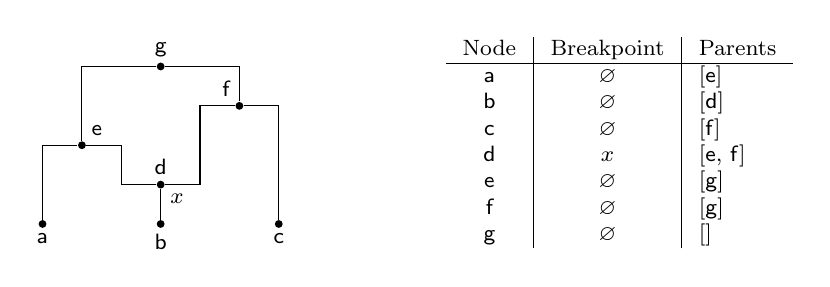
\begin{tikzpicture}[x=5mm, y=5mm, node distance=2mm and 20mm]
\tikzset{greynode/.style={circle,fill,inner sep=1},
nodelabel/.style={font=\footnotesize}}

\node (s0) [greynode] at (0, 0) {};
\node (s1) [greynode] at (3, 0) {};
\node (s2) [greynode] at (6, 0) {};
\node (s3) [greynode] at (3, 1) {};
\node (s4) [greynode] at (1, 2) {};
\node (s5) [greynode] at (5, 3) {};
\node (s6) [greynode] at (3, 4) {};

% \node [anchor=north west] at (0,6) {A};
\node [nodelabel,anchor=north west] at ($(s3) + (0,0)$) {$x$};
\foreach \u/\lab in {s0/$\textsf{a}$, s1/$\textsf{b}$, s2/$\textsf{c}$} \node[nodelabel,anchor=north] at (\u) {\lab};
\foreach \u/\lab in {s4/$\textsf{e}$} \node[nodelabel,anchor=south west] at (\u) {\lab};
\foreach \u/\lab in {s5/$\textsf{f}$} \node[nodelabel,anchor=south east] at (\u) {\lab};
\foreach \u/\lab in {s3/$\textsf{d}$, s6/$\textsf{g}$} \node[nodelabel,anchor=south] at (\u) {\lab};

%% Edges
\draw (s1) -- (s3);
\draw (s0) |- (s4);
\draw (s4) -- (2,2) |- (s3);
\draw (s4) |- (s6);
\draw (s3) -- (4,1) |- (s5);
\draw (s2) |- (s5);
\draw (s5) |- (s6);

% \node [anchor=north west] at (9,6) {B};
\node [nodelabel,anchor=north west] at ($(10,5)$) {
\begin{tabular}{c|c|l}
% \multicolumn{2}{c}{Breakpoints}\\
Node & Breakpoint & Parents\\
\hline
$\noderef{a}$ & $\varnothing$ & [\noderef{e}]\\
$\noderef{b}$ & $\varnothing$ & [\noderef{d}] \\
$\noderef{c}$ & $\varnothing$ & [\noderef{f}]\\
$\noderef{d}$ & $x$ & [\noderef{e}, \noderef{f}] \\
$\noderef{e}$ & $\varnothing$ & [\noderef{g}]\\
$\noderef{f}$ & $\varnothing$ & [\noderef{g}]\\
$\noderef{g}$ & $\varnothing$ & []\\
\end{tabular}};

% \node [anchor=north west] at (9,6) {C};
% \node [nodelabel,anchor=north west] at ($(10,5)$) {
% \begin{tabular}{ll}
% Edges & Intervals\\
% \hline
% $(\textsf{a}, \textsf{e})$ & $(0, L]$ \\
% $(\textsf{b}, \textsf{d})$ & $(0, L]$ \\
% $(\textsf{c}, \textsf{f})$ & $(0, L]$ \\
% $(\textsf{d}, \textsf{e})$ & $(0, x]$ \\
% $(\textsf{d}, \textsf{f})$ & $(x, L]$ \\
% $(\textsf{e}, \textsf{g})$ & $(0, L]$ \\
% $(\textsf{f}, \textsf{g})$ & $(0, L]$ \\
% \end{tabular}};

\end{tikzpicture}
\caption{\label{fig-arg-data-structure}
A graphical depiction of a classical event ARG and a concrete
encoding of the information. Node \noderef{d} is a recombination
event as it is associated with a non-null breakpoint, and has
two parents. Nodes \noderef{e}, \noderef{f} and \noderef{g} are
common ancestor events.
}
\end{figure}

In keeping with its original derivation in terms of a stochastic
process (see Appendix~\ref{sec-arg-history}), the classical definition of an
ARG data structure is
in terms of events.
Nodes represent
common ancestor or recombination events that occurred in the
history of some set of sample genomes, and edges represent ancestral
lineages~\citep{griffiths1996ancestral}.
In a common ancestor event the inbound lineages are merged into a
single ancestral lineage, and in a recombination
event a lineage is split into two independent
ancestral lineages.
% The final vital
% detail is that we associate a breakpoint with each recombination
% event.
% This information is sufficient to uniquely
% define the local genealogical trees at every position along the genome,
% which is the basic requirement for a data structure encoding
% genome-wide genetic ancestry.
As illustrated in Fig.~\ref{fig-arg-data-structure}, this information
is usually concretely encoded by associating a recombination breakpoint
(which is null for common ancestor events) and an ordered list of parents
with each node. We refer to such a  data structure as an
``event ARG'' (eARG).
To recover the local tree at genome coordinate $x$ (the most
fundamental operation required for an ARG data structure),
we traverse the graph rootwards from the leaves.
At a particular
node $u$, if it has one parent we are at a common ancestor
node and we follow that parent. If we are at a
recombination node, $u$ has two parents: if
$x$ is less than the breakpoint we follow
the edge to the first parent, and otherwise follow the edge
to the second parent.
The order in which parents are listed at a recombination node is
therefore significant, telling us
from which parent the segments of genome to the left and right of the breakpoint
were inherited.

[TODO list the salient points that we want to contrast against
the gARG. We don't want this to seem like a straw man]

% \section*{Inheritance and ancestral material}\label{Ancestry_resolution}
\section*{Prospective vs restrospective ARGs}
ARGs are usually thought of as a restrospective structure, in which we
reason about the genomes that are genetic ancestors of some set of
sample genomes. Figure~\ref{fig-arg-in-pedigree}
is retrospective because it only includes information
about genetic inheritance relative to the sample individuals
$I_1$ and $I_2$ (genomes \textsf{a}--\textsf{d}).
Genetic inheritance must have occured between (e.g.)
$I_8$ and her daughter $I_6$, but this is not recorded because
% this is probably not true, given we know the complete pedigree?
we have no information about it, given these samples.
Event ARGs, given their roots in the coalescent with recombination,
are inherently retrospective. They define the evolutionary
events that have occured in the genetic ancestry of a sample.
% This is weak, rephrase.
An event ARG must have some set of samples, or there
will be nothing to define events in terms of.

The gARG representation, on the other hand,
can be either retrospective or \emph{prospective}.
The edges in a gARG represent a path of genetic inheritance from
ancestor to descendant through some
number of generations (ultimately from cell to cell),
and are annotated
with the genome coordinates over which inheritance occurs.
In a prospective gARG, the inheritance intervals $I$
on an edge joining ancestor genome $v$ and descendant $u$
defines \emph{all} regions of genome that $u$ inherited from $v$.
Thus, these  inheritance intervals are
concerned only with the genetic relationship
between the nodes in question, and are not defined with respect
to any given set of samples. We are simply recording the
direct genetic inheritance between two genomes
(in the simplest case, between a parent and a child).

Prospective ARGs occur in individual-based forwards-time
simulations~\citep{kelleher2018efficient,haller2018tree},
where the genetic inheritance between genomes is recorded
exhaustively and periodically
``simplified'' to retain only
the ancestry relevant to the current population.
\citet{kelleher2018efficient} refer to the structure
recording all such forwards-in-time genetic relationships
as an ``embellished pedigree`` (and suggest the term ``nedigree''
as a shorthard).
Describing this instead as a ``prospective ARG'', emphasising
the use of the same data structures and the direct connection with
the usual retrospective interpretation of an ARG, may be
more useful.
The ``simplify'' algorithm which converts a prospective
gARG into a retrospective one is a powerful tool,
with several other applications
as we discuss in the following sections.

\section*{Converting an eARG to a gARG}
The process of converting an eARG to a gARG is very similar to
simplifying a prospective gARG with respect to a set of samples,
and highlights some important differences between the encodings.
The process involves two steps, and is illustrated in
Fig~\ref{fig-ancestry-resolution}.

\begin{figure}
\centering
% TODO update the source of this figure to make less tall. It's taking
% up far too much vspace at in native coords at the moment.
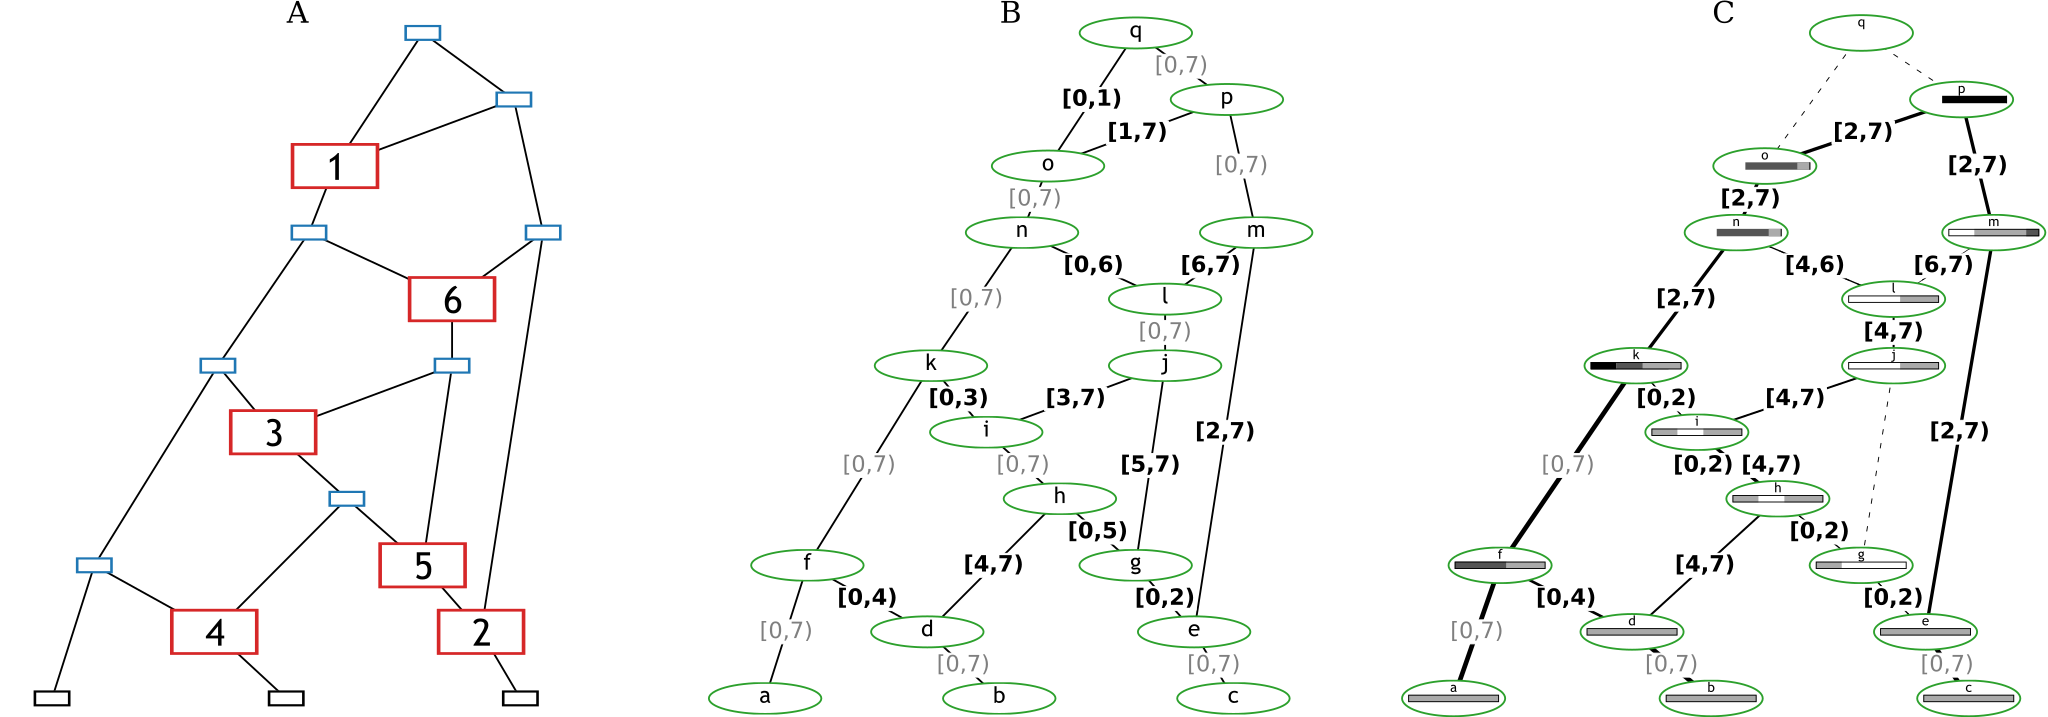
\includegraphics[width=0.75\textwidth]{illustrations/ancestry-resolution}
\caption{\label{fig-ancestry-resolution}
Converting the \citet[][Fig.~1]{wiuf1999recombination} example graph
to a gARG. (A) The original eARG; square nodes represent events, with
each recombination (red) showing the corresponding breakpoint.
(B) The corresponding gARG with breakpoints directly converted to
edges annotated with inheritance intervals.
(C) The sample-resolved gARG resulting from simplifying with respect
to the samples, $a$, $b$, and $c$. Dashed lines show edges that are
no longer present (in practice, nodes $g$ and $q$ would also be removed).
Coalescence with respect to the sample is indicated by shaded bars, as
in Fig~\ref{fig-arg-in-pedigree}A.
Line thickness is proportional to the genomic span of each edge.
Nodes representing recombination events have been retained
for clarity, but could be removed by simplification if
desired.
}
\end{figure}

The first step is straightforward
(Figure~\ref{fig-ancestry-resolution}B).
We duplicate the nodes and
edges from the input eARG, and the add inheritance annotations
to the output gARG's edges. If the node is a common ancestor node,
we annotate the single outbound edge with the interval $(0,L]$.
If the node is a recombination node with a breakpoint $x$,
we annotate the outbound edges with the intervals $(0, x]$
and $(x, L]$.
These inheritance annotations are clearly in one-to-one
correspondance with the information in the input eARG,
but they are a superset of the
``ancestral material''~\citep{wiuf1999ancestry,wiuf1999recombination}
of the sample.

Ancestral material is a critical concept in a retrospective ARG,
and refers to the genomic intervals directly ancestral to the samples
scattered across lineages (the edges of the graph)
at some time in the past. At recombination
events, ancestral material is split between the ancestral lineages.
As genome segments coalesce in a common
ancestor the total amount ancestral material is reduced, until
eventually as we traverse pastwards through the graph, all
samples reach a most recent common ancestor at all locations
along the genome. The process of transmitting ancestral material
along the edges of an ARG is directly analogous to Hudson's
simulation algorithm for the coalescent with
recombination~\citep{hudson1983testing,kelleher2016efficient}.

Fig~\ref{fig-ancestry-resolution}C shows the graph that we obtain
by resolving the ancestral material transmitted along each edge
(using the ``simplify'' algorithm), and highlights some important
differences between the eARG and gARG encodings.
Firstly, we can see that some nodes and edges are removed entirely
from the graph. The ``grand MRCA'' $q$ is ommitted from the
fully resolved gARG because all segments of the genome have
fully coalesced before it is reached. Likewise, the edge
between $g$ and $j$ is omitted because the recombination
event at position $5$ fell in non-ancestral material.
More generally, we can see that the fully resolved
gARG encoding of Fig~\ref{fig-ancestry-resolution}C
allows for ``local'' inspection
of an ARG in a way that is not possible by storing
common ancestor and recombination events in an eARG. Because
the ancestral material is stored with each edge, the effects
of multiple events can be reasoned about at once. Many algorithms
that we wish to perform on an ARG will require resolving
the genetic material with respect to a sample.
% this is weak, but would be good to emphasise this point.
% you just end up running simplify lots of times, in your
% downstream algs
The gARG encoding
allows us to do this once and to store the result, whereas
the eARG encoding requires us to repeat the process on
each traversal.

It is important to note here that the \citet{wiuf1999recombination} eARG
example used here is something of a straw man, in that it is highly unlikely
that an inference or simulation program would produce a retrospective
ARG that contains
nodes or edges that are not ancestral to the sample. Nonetheless, it
is an instructive example from the literature which highlights several
important properties of ARGs, and the general point about
the need to resolve ancestral material ``on the fly'' for eARG traversals
holds.


%(see Appendix XXX) and has several features that we are unlikely to simulate or
%infer in practice. For example, by definition the samples contain no genetic information about
%nodes \textsf{g} and nodes \textsf{j} and so neither of those nodes are likely to be inferred.
%Likewise, is is unlikely we would have information to infer the ``grand MRCA''
%\textsf{q} as all regions of the genome have already reached a
%common ancestor separately (in nodes \textsf{k} and \textsf{p}).

% Third, there exist nodes such as
% \textsf{k} with two children (i.e. ``common ancestor'' nodes in Hudson's terminology)
% but in which no ancestral coalescence occurs. Fourth, some breakpoint positions occur
% within regions of genome that are not ancestral (e.g. the breakpoint at position 3 in
% node \textsf{k}). In this case sample-resolved edge annotations lose the exact position of
% the breakpoint, although they retain the information that a breakpoint occurred between
% positions 2 and 4 (which is sufficient for calculating the likelihood, see appendix XXX).


% reduce the annotation intervals to those that are ancestral to the
% sample (note that node $q$ is now ommitted because the MRCA of the sample
% has already been found for the full genome at node $p$).
% Tracking such
% ``ancestral material''~\citep{wiuf1999ancestry,wiuf1999recombination}
% is much more useful~\citep{mcgill2013graphml,arenas2013importance}
% and, indeed, all that is possible to
% have information about when inferring ARGs from contemporary samples.
% We refer to a gARG with inheritance annotations of this type as
% ``sample resolved''.

% Fig~\ref{fig-ancestry-resolution} is an instructive example
% from the literature \citep{wiuf1999recombination} and illustrates
% how a classical eARG (Fig~\ref{fig-ancestry-resolution}A) can be described as
% a gARG with edge annotations (Figs~\ref{fig-ancestry-resolution}B~and~C).

% There are two distinct annotation schemes possible, and the distinction is subtle
% and important. The first scheme is to use the annotations to describe the complete
% set of genomic intervals directly inherited by the descendant node from the ancestor
% node (Fig~\ref{fig-ancestry-resolution}B). The second is to use the edge annotations to
% describe the ``ancestral material''~\citep{wiuf1999ancestry,wiuf1999recombination}
% of the sample that is propagated through
% the graph from descendant to ancestor (Fig~\ref{fig-ancestry-resolution}C).
% As we discuss in section XXX, this second scheme has many advantages
% in terms of efficiency.


%ARGs are inherently a retrospective structure defined in terms
%of a set of sample nodes (usually the leaves), and,
%as we discuss in section XXX, storing sample-resolved ancestry
%intervals (Fig~\ref{fig-ancestry-resolution}C) is generally much more
%useful than storing the parent-child intervals recording direct inheritance
%(Fig~\ref{fig-ancestry-resolution}B).
%Indeed, storing direct inheritance intervals for edges is really only of interest because of
%its correspondence with the classical approach of associating
%breakpoints with recombination nodes in an eARG (Fig~\ref{fig-ancestry-resolution}A).
%The eARG encoding is simply a more limited form, in which the only types of direct
%inheritance we can have are the entire genome, or the intervals
%at either side of a recombination breakpoint.

%Note that this example is a sample from the so-called \emph{``big'' ARG process}
%(see Appendix XXX) and has several features that we are unlikely to simulate or
%infer in practice. For example, by definition the samples contain no genetic information about
%nodes \textsf{g} and nodes \textsf{j} and so neither of those nodes are likely to be inferred.
%Likewise, is is unlikely we would have information to infer the ``grand MRCA''
%\textsf{q} as all regions of the genome have already reached a
%common ancestor separately (in nodes \textsf{k} and \textsf{p}).

% Third, there exist nodes such as
% \textsf{k} with two children (i.e. ``common ancestor'' nodes in Hudson's terminology)
% but in which no ancestral coalescence occurs. Fourth, some breakpoint positions occur
% within regions of genome that are not ancestral (e.g. the breakpoint at position 3 in
% node \textsf{k}). In this case sample-resolved edge annotations lose the exact position of
% the breakpoint, although they retain the information that a breakpoint occurred between
% positions 2 and 4 (which is sufficient for calculating the likelihood, see appendix XXX).

% Given a gARG with direct-inheritance edge annotations
% (Fig~\ref{fig-ancestry-resolution}B),
%  we obtain the sample-resolved edge annotation
% (Fig~\ref{fig-ancestry-resolution}C) by traversing the graph backwards in time
% from sample nodes (\textsf{a}, \textsf{b}, \textsf{c}).
% Proceeding in topological order (such that an ancestor node is visited
% after all of its descendants) the sample-resolved material for a node is the
% union of the sample-resolved intervals on its inbound edges. We then annotate
% the outbound edges with the intersection of their direct-inheritance intervals
% and the just-computed sample-resolved intervals for the node.
% For example, node \textsf{i} in Fig~\ref{fig-ancestry-resolution}C
% carries sample-resolved material on the intervals $(0, 2]$ and $(4, 7]$. The edge
% joining \textsf{i} to its ancestor \textsf{k} then carries
% material on $(0, 2]$ since although \textsf{i} directly inherits interval
% $(0, 3]$ from \textsf{k} (Fig~\ref{fig-ancestry-resolution}B), only $(0, 2]$ is
% ancestral to the sample. For each node, we also keep track of the number of
% descendant samples over each genomic interval, and stop tracking that
% interval once the lineages from all samples have coalesced. For example,
% the edge from \textsf{k} to \textsf{n} omits the region $(0,2]$ because it has
% already fully coalesced (indicated by a fully black genomic region).


% In practice, the backwards-in-time Griffiths process that produces
% ARGs such as that shown in Figs~\ref{fig-ancestry-resolution}A~and~B
% is rarely simulated, because the resulting ``big ARG'' (Appendix XXX) is
% dominated by nodes such as \textsf{g} and \textsf{j} which contain information
% about inheritance in non-ancestral material, as well as nodes such as
% \textsf{o} and \textsf{q} which track details of ancestry even once the
% local genomic region has fully coalesced. Instead, simulating
% ARGs from the coalescent with recombination is usually done by
% running Hudson's algorithm to produce a sample-resolved ARG directly.
% Moreover, when inferring ARGs from genetic data, there is no information
% in the sample set that can be used to resolve these nodes, so that they
% are essentially unknowable.

% The process of converting a gARG with local-inheritance annotations
% to its sample-resolved equivalent is also known as ``simplification'',
% and is the key algorithm underlying recent
% advances in forwards-in-time
% simulation~\citep{kelleher2018efficient,haller2018tree}.
% It has many useful properties, as we discuss in the next section.

% It is worth noting the process of sample resolution can reveal that certain ARG
% nodes are \emph{redundant}: if they are removed and the edges adjusted to
% pas directly from the node's child to the node's parent, it does not reduce our
% knowledge of the samples' genetic ancestry. Removing nodes,
% both redundant ones and others, is part of a process we call
% ``simplification''.

\section*{Levels of simplification}\label{ARG_simplification}
ARG simplification is a powerful tool, and can do much more
besides removing unreachable nodes and edges in a prospective ARG
and resolving ancestral material in an eARG.
In general, we can think of
ARG simplification as the process
of removing nodes and re-writing edges in a gARG to remove
various types of redundancy.
Many of the types of redundancy revolve around the presence
of ``unary'' nodes in the local trees
(a tree node that has exactly one child).

Fig.~\ref{fig-simplification} show a series of successive steps of
simplification, starting with a complete gARG simulated under a
backwards-in-time Wright-Fisher
model, shown both as a graph on the left, and the corresponding sequence of 6
local trees on the right.
For example, consider the path above node
\textsf{a} in the first tree (covering positions 30 to 40)
in Fig.~\ref{fig-simplification}A.
Before \textsf{a} meets its common ancestor with the other samples at
node \textsf{q}, it passes through \textsf{e}, \textsf{j}, \textsf{m}, \textsf{n} and
\textsf{p}, which in this region of the genome are all unary nodes.
This reflects the passage of this span of genome through the ARG towards the root.
Such unary nodes in a local tree are not usually considered important;
% because they provide little information and are not
% detectable by information from any given individual tree.
nodes usually mark the points where samples coalesce in a
 \emph{common} ancestor. For most purposes, we would therefore consider a path directly
joining sample \textsf{a} to node \textsf{q} to be equivalent to the path
containing the intermediate unary nodes.

\begin{figure}
\centering
\vspace{5em}
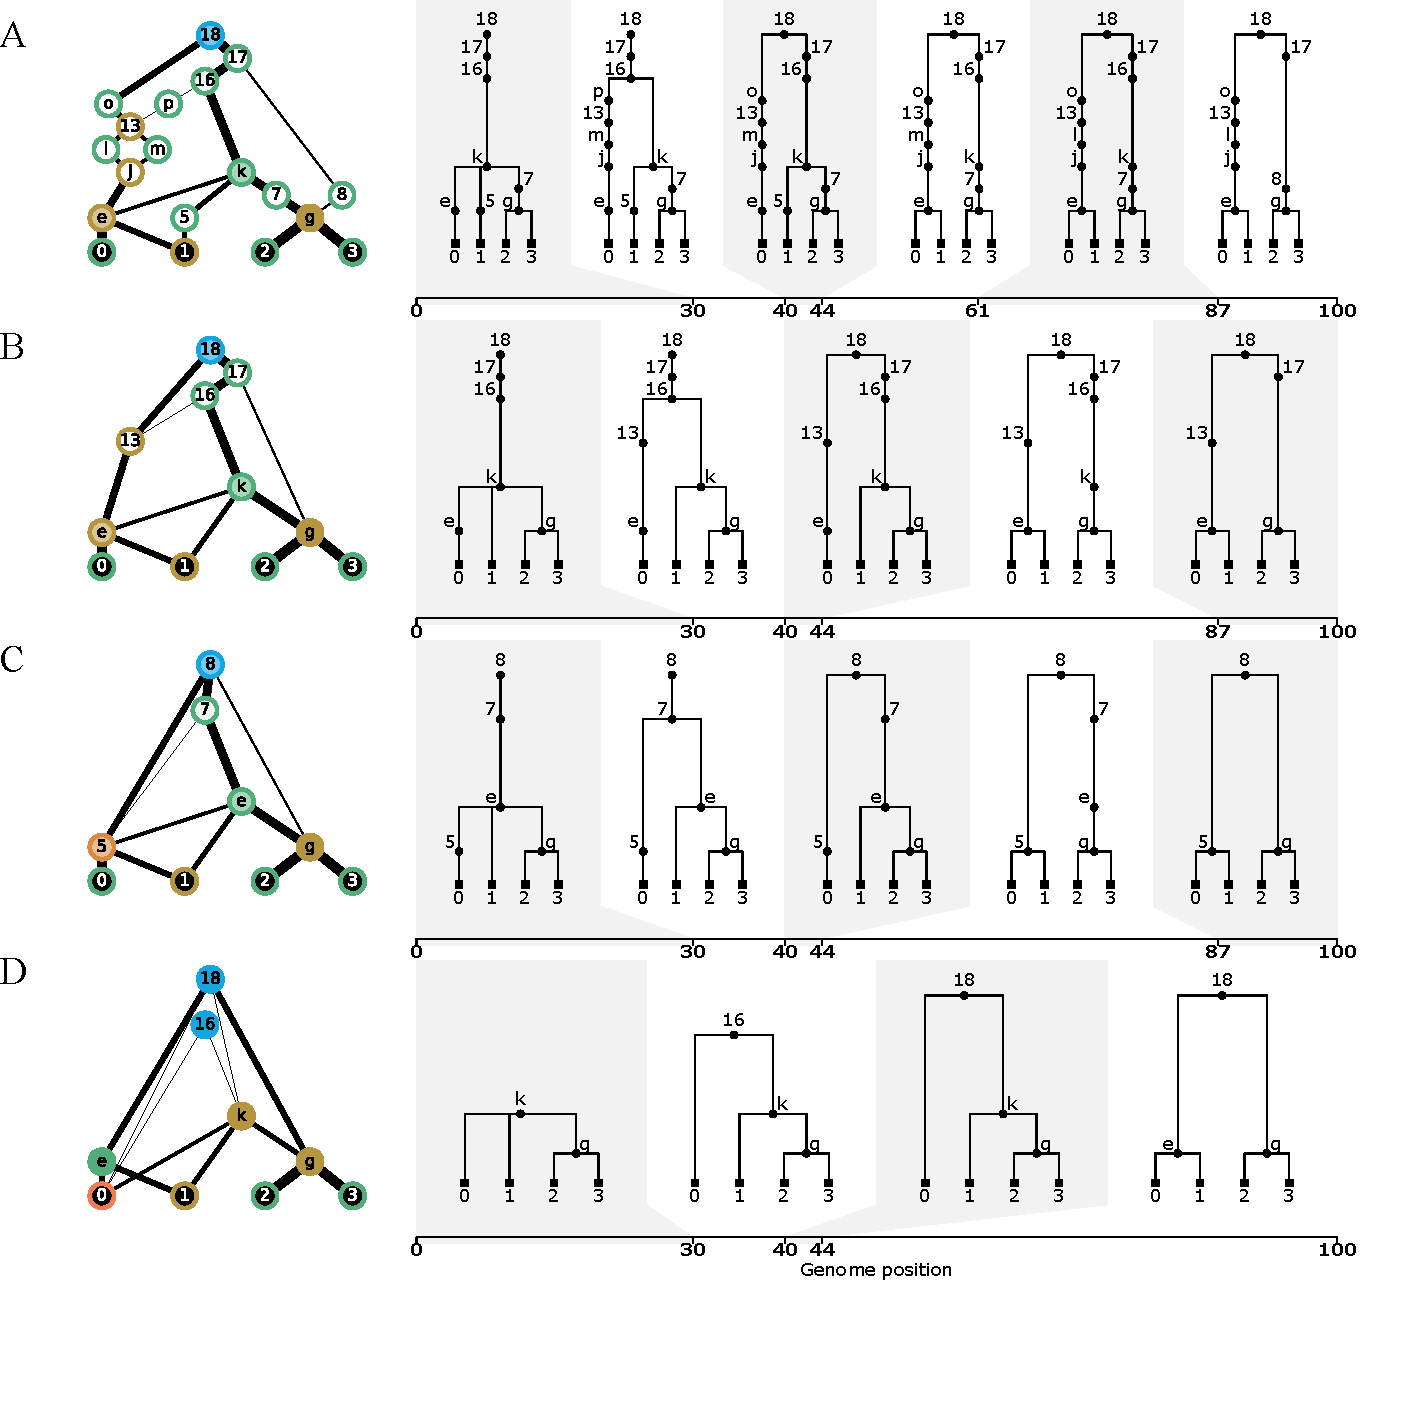
\includegraphics[width=\linewidth]{illustrations/simplification}
\caption{\label{fig-simplification}
Levels of ARG simplification.
In all cases the graph visualization is shown on the left
and the corresponding local trees on the right.
Nodes are coloured by the number of parents and shaded
according to the proportion of their span over which they are coalescent.
(A) A gARG simulated from a diploid Wright-Fisher
model. Note that the genome \textsf{k} has three children, and the genomes
\textsf{e} and \textsf{g} simultaneously have multiple parents and multiple
children.
(B) Simplified to remove all
% trying out this terminology - can define in the text
1-connected graph components (e.g., diamonds such as \textsf{jlnm}).
(C) Remove nodes that are unary in all local trees. This removes both recombinant nodes
that have only one child (e.g. \textsf{n}) and nodes that have more
than one child (i.e. are ``common ancestors'') but never represent coalescences
in the local trees (e.g. \textsf{r}).
(D) Rewrite edges to bypass any unary nodes in local trees. Note that this loses lineage
information such as the fact that \textsf{k} is connected to \textsf{a} via \textsf{e}.
}
\end{figure}

The first level of simplification that we can perform is to remove
graph topology that is invisible to the samples.
An example of such topology is a
``diamond''~\citep{rasmussen2014genome}
in which the two parent nodes of a recombination immediately
join again into a common ancestor (e.g.~\textsf{j}, \textsf{l}, \textsf{m}
and \textsf{n} in Fig.~\ref{fig-simplification}A).
Unless we are specifically
interested in the recombination event or these ancestral genomes,
there is no information in this topology and the diamond can be
replaced by a single edge. More generally, any
subgraph that is singly-connected in both the leafward and
rootward direction (a ``super-diamond'') is non-identifiable and can be
replaced by one edge. This definition includes the case
of a node that has one inbound and one outbound edge, such as
nodes \textsf{f} and \textsf{h}.
Fig.~\ref{fig-simplification}B shows the result of this type of
graph topology simplification.

Simplifying away diamonds will remove many unary nodes from the
local trees, but there can still be nodes that are unary in all
of the local trees. In particular, a node can represent a recombinant
with multiple parents in the graph but only a single child (e.g.\ node \textsf{n}
in Fig.~\ref{fig-simplification}B), or can represent a common ancestor with
multiple children in the graph but in which no coalescence takes place
in the local trees
(node \textsf{r} in Fig.~\ref{fig-simplification}B).
% point out that this is why Hudson refers to CA nodes, not coalescence nodes
Such nodes are not singly connected in the graph, but are nevertheless unary in
all of the local trees.
The operation to remove them
therefore requires knowledge not just of the graph topology but also of the
ancestral material associated with the edges.
As we see in Fig.~\ref{fig-simplification}C,
removal of recombinant nodes can produce graph nodes with
more than two parents (e.g.~node \textsf{e}); and likewise, removal of
common ancestor but non-coalescent nodes can produce graph nodes with
more than two children (e.g.~node \textsf{s}). These represent a ``stacking up'' of
multiple---often indistinguishable---events into a single node.
% something which is impossible to encode in an eARG.

% JK: Text moved from an earlier section. See if we want to reuse this here
% if not already said.
% Indeed a single node can have both multiple children
% and multiple parents. This would be the case in Fig~\ref{fig-arg-in-pedigree} if,
% for instance, node \textsf{a} were to have two children.
% % It is a shame that this is not actually shown in fig 3, but I don't think
% % we can do this unless we have 5 generations
% Moreover, a single node can have more than 2 children, and (as we shall see in
% the ``\nameref{ARG_simplification}'' section), more than 2 parents. Another way to
% state this is that transitions between nodes in a gARG can encapsulate multiple
% events in an eARG.

The remaining nodes are MRCAs of some subset of the samples
at \emph{some} positions along the genome. We still have
some unary nodes in the local trees, but these nodes will
correspond to a coalescence in at least one other
local tree. For example, node  \textsf{k} is unary in the second tree
of Fig.~\ref{fig-simplification}C, but is either binary
or ternary in all subsequent trees (recall this is a Wright-Fisher
simulation). The final level of simplification is to alter the edge annotations
such that, although no nodes are removed from the graph, all
unary nodes disappear from the local trees (Fig.~\ref{fig-simplification}D).
Note that although this last stage produces simpler local trees, by
removing information about the exact paths taken by lineages through
the graph, we lose potentially useful information about shared edges
between trees. The extent to which this information can be inferred
and utilised is an interesting open question.

An important consequence of simplifying ARGs to remove
unary nodes in local trees is that we lose some information
about recombination
events. This is related to the amount of \emph{precision} about
recombination events that we store, which is the topic of the next
section.

\section*{Precision of recombination information}
% The ARGs in Fig.~\ref{fig-simplification} represent different
% levels of detail about the same ancestral history. They represent
% the same set of recombination and common ancestor events,
As illustated in Fig.~\ref{fig-simplification}, successive levels
of ARG simplification reduce the amount of information about the
history of the sample that is stored. Some of the information lost,
for example, ``diamond'' removal (Fig.~\ref{fig-simplification}A),
seems like a reasonable tradeoff for a simpler structure.
The consequences of other simplifications, however, are
more subtle and relate directly to what can be known about
recombination events and the levels of precision that
we should seek to infer about them.

The ARGs in Fig.~\ref{fig-simplification} contain different
numbers of local trees ($6$, $5$, $5$ and $4$ for A through
D, respectively). When we move from A to B the local trees
for the intervals $(44,61]$ and $(61,87]$ are merged because
the only differences between them are their journeys through
nodes \noderef{l} and \noderef{m}. These nodes that participated
in the diamond are removed from the ARG, and we have lost
all information about the corresponding recombination at
position 61. Other nodes (e.g.\ \noderef{o} and \noderef{p})
have also been removed but these represent the \emph{parents}
of recombinants. The recombinant nodes themselves
(e.g. \noderef{n}) are still present, and represent precise
information about the time, genomic location and tree
branches involved
in the recombination event.

Fig.~\ref{fig-simplification}C has the same number of local trees
as Fig.~\ref{fig-simplification}B, but has less precise information
about recombination. Continuing the previous example, node
\noderef{n} has been removed from the graph because it was unary
in all of the local trees; its outbound edges to \noderef{s}
and \noderef{q} have effectively been ``pushed down''
to \noderef{e} (which is retained because it is the coalescent
parent of \noderef{a} and \noderef{b} over the interval
$(44, 100]$). We
have therefore lost precision about
the \emph{timing} of this recombination event, and know only
that it must have occured between the times of node \noderef{e}
and \noderef{q}.

Fig.~\ref{fig-simplification}D removes all unary nodes from the
local trees, and further reduces the precision of
recombination information. Node \noderef{e} has not been
removed from the graph because it is coalescent in the
final tree, but we no longer know that the recombination
event at position 30 was ancestral to it, or have
any indication of its timings. Furthermore,
trees for $(44, 87]$ and $(87, 100]$ were only distinguishable
by the passage of the former tree through nodes \noderef{e}
and \noderef{q}, and so the recombination on node \noderef{g}
at position 87 has been lost entirely.

% The example in Fig.~\ref{fig-simplification} is usually
% referred to as ``fully simplified'', and is the default output
% of simulation programs like \msprime. While there is significant
% precision about recombination events lost

The point of these examples is to emphasise that
information about recombination in an ARG is not ``all
or nothing'': there is a continuuum of detail
about recombination, in terms of genomic location, timing
the ancestral lineages involved, that we can describe.
While there has been a recent tendancy to emphasise the
importance of ``full ARGs''
\citep[e.g.][]{deng2021distribution,brandt2021evaluation,
rasmussen2022espalier}
which contain complete information about all recombination
events, it is reasonable to question the value of
such precise information and whether it is knowable.
[SOME MORE STUFF]

% Ancestral recombination graphs are often characterised
% as consisting of a complete record of the genetic history
% of a sample. For example,
% \cite{rasmussen2014genome} state that an ``ARG provides a record of all
% coalescence and recombination events since the divergence of the sequences
% under study'' and
% according to \cite{deng2021distribution} an ARG
% ``provides all the information about the genealogical history of a sample,
% including the locations of recombination events.'' It is worth
% questioning, however, whether such comprehensive information
% will always be available, and in particular whether our
% representation of genealogical history should \emph{require}
% such precision. Simulations will usually generate complete
% information about the history of a sample, of course, but
% we may not have sufficient information to infer such detail.

% % The full ancestral recombination graph (ARG) is a structure that encodes all
% % coalescence and recombination events resulting from the stochastic process of
% % the coalescent with recombination.
% \citet{brandt2021evaluation} define a ``full'' ARG as
% ``a structure that encodes all
% coalescence and recombination events resulting from the stochastic process of
% the coalescent with recombination'' (thus going against the general
% historial trend discussed in the XXX section).
% \citet{rasmussen2022espalier} have a less restrictive definition, in
% which a ``full'' ARG is one that contains complete information about
% recombination events, without necessarily being tied to a particular
% stochastic process.
% While [something positive], it is important to be clear on
% what the overall goal of such precise inferences are,
% what the limitations on when they can be made are,
% and their downstream utility in applications.

% % What is the goal of having fully precise ARGs?
% % 1) studying the actual recombination events;
% % 2) evaluating the likelihoods
% The main reasons for wanting precise estimates of all recombination
% events are to either compute a likelihood of the inferred ARG
% under a statistical model, or to study the recombinants in
% detail~\citep{rasmussen2022espalier}.
% % Explain that we're really interested in the details of recombination
% % itself with a small number of samples.
% In the latter case, we might
% have a small number of samples~\citep{guo2022recombination}.

% Beyond cases in which visual inspection of the trees and the
% effects of recombination is feasible, the main application
% of having completely precise estimates of recombination events is
% to evaluate the likelihood of the estimate under some
% statistical model. The only statistical model available
% is the coalescent with recombination
% and its approximations~\citep{mcvean2005approximating,marjoram2006fast}.
% In this case, the utility of a ``full`` ARG for some dataset
% is limited by how well the dataset fits the assumptions
% of the model.

% % Not sure where this goes, but there are some critical points
% % that we want to explain and not just throw out there in the
% % discussion.
% % A critical distinction between the eARG and gARG encodings
% % is the level of precision about the time and location of
% % recombination events that is required. In an eARG, we are
% % required to be absolutely precise about every recombination
% % [explain and contrast with gARG, referring to examples]

% % JK: This is very rough, just jotting down the basic ideas,
% % will need substantial revision.
% It is not clear that such complete information will always
% (or indeed ever) be available from inferences~\cite{shipilina2022origin}.
%  We may be
% able to precisely identify the location and timing
% of recent recombinations (particularly if detailed pedigree
% information is available) but beyond this, the information
% required simply isn't present. When sampling from a
% process such as the Sequentially Markov
% Coalescent~\citep{mcvean2005approximating,marjoram2006fast}
% like ARGweaver~\citep{rasmussen2014genome}, it is true that
% we do obtain a fully resolved ARG with precise
% information about recombination, but it is reasonable
% to question how much information from the data is used
% to support older recombinations, in particular.

% % This idea of a continuum of information about recombination
% % being inferrable and representable is consistent with the ideas
% % discussed by~\cite{shipilina2022origin}. There a haplotype block
% % is synonymous with coalescent nodes in the ARG, which we can generalise
% % as nodes in a gARG with at least two children. In principle, these
% % nodes are identifiable by the mutations that occur on the outbound
% % edges of the node.

% It is helpful to consider the difference between fully
% resolved binary trees and those that contain polytomies.

% The situation is in fact directly analogous: an ARG that
% contains fully resolved recombination information must have
% at most parents per node.

% At the very least, it is not reasonable for the \emph{data
% structure} to require complete precision in order to
% represent some less precise. This is a fundamental
% advantage of the gARG encoding over the classical eARG
% method: we are not forced to posit a precise cause (recombination
% event) for every effect (difference between adjacent trees).
% These differences in precision of recombination
% information are illustrated in the ARGs estimated by different
% methods, as we see in the next section.

% In general, discussions tend to contrast an ARG
% on one hand as holding \emph{complete} information about recombination
% (and therefore between-tree correlation structure)
% and a sequence of local trees on the other (with, by implication,
% no direct information about between-tree correlations).
% This is a false dichotomy:
% a \emph{continuum} of information about recombination and between-tree
% correlation structure can be represented and inferred, and all
% such levels of information are useful, even if only for computational
% efficiency.


\begin{figure} \begin{center}
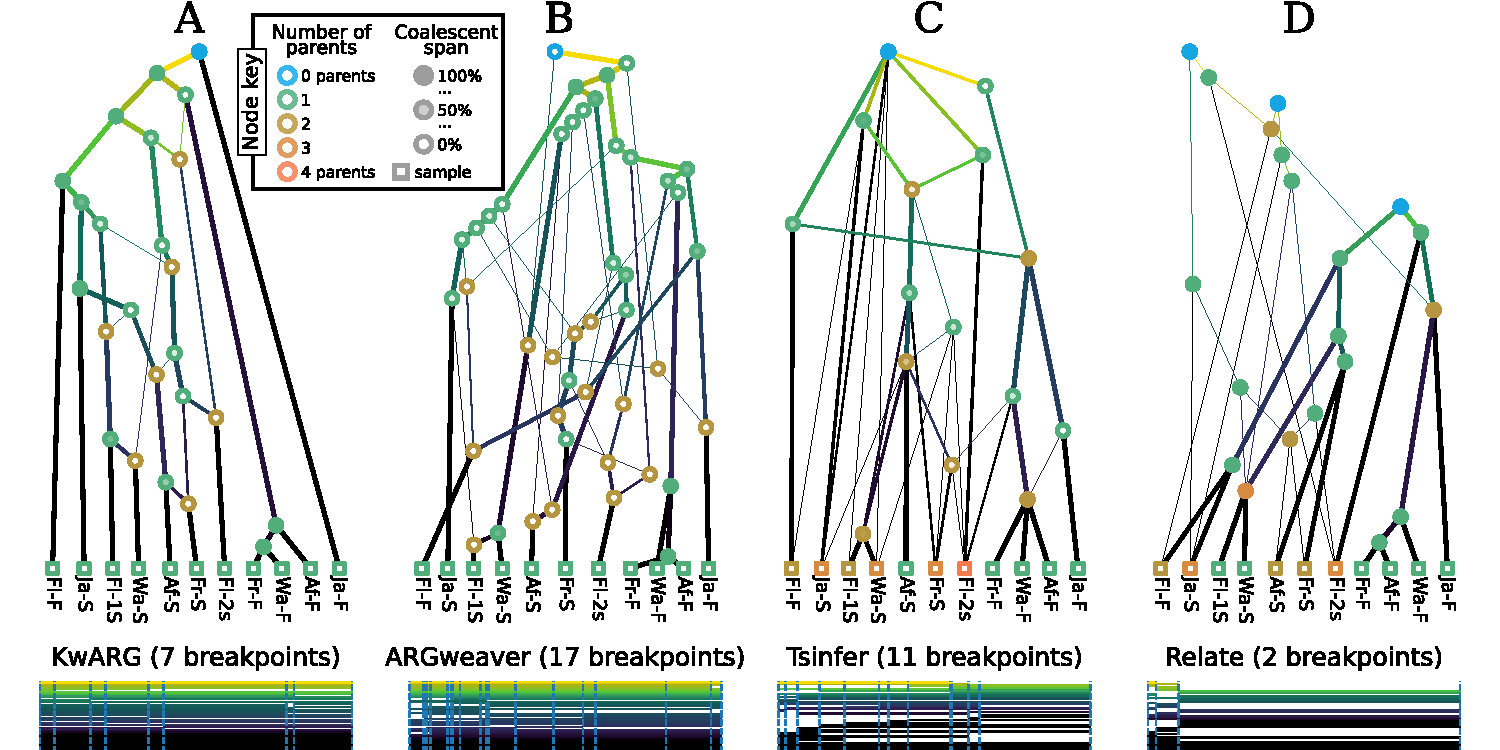
\includegraphics[width=\textwidth]{illustrations/inference.pdf} \end{center}
\caption{\label{fig-inferred-args} ARGs inferred by
(A) \kwarg~\citep{ignatieva2021kwarg},
(B) \argweaver~\citep{rasmussen2014genome,hubisz2020inference},
(C) \tsinfer~\citep{kelleher2019inferring},
and (D) \relate~\citep{speidel2019method}
for 11 samples of a 2.7kb region of the \textit{Drosophila melanogaster} ADH
locus~\citep{kreitman1983nucleotide}. The \argweaver\ example
is a sample from the inferred posterior distribution. In each ARG,
colours are assigned to edges based on the time of the edge's child node:
lighter colours are assigned to edges with older child
nodes, darker colours are assigned to edges with younger child nodes
Note that the position of points on the
Y axis is chosen for graphical clarity by the graphviz \texttt{dot}
algorithm, rather than as a direct measure of time.
Line width corresponds to the genomic span of the edge. Node colour
refers to the number of parents of the node: red is zero, brown is one,
green to blue are two to N parents. The brightness
of the node is determined by the genomic span over which
the node has two or more children divided by the span where it has any
children. The genomic intervals associated with edges are visualised below
each ARG, where each row is an edge
and the x axis reflects genomic position. The width of edges
thus corresponds to their genomic span. Edges
are ordered by the age of their child node, from oldest to youngest
moving down the page, with colours matching the edge colours in the ARG.
Vertical lines indicate breakpoints between local trees.
}
\end{figure}

To illustrate these points and to emphasise the heterogeneity
of the ARGs inferred by current methods, we inferred ARGs for the
the classical \citet{kreitman1983nucleotide} benchmark dataset
using four recent inference methods and show the results in
Fig~\ref{fig-inferred-args}.
While there is some consistency among the inferred ARGs (such as the samples
FR-F, WA-F and Af-F being grouped into the same clade), there
are also considerable differences. For this dataset, the minimum number
of recombination breakpoints required in the absence of recurrent mutation
is 7~\citep{song2003parsimonious}, and the number of inferred breakpoints
under the input mutation and recombination rates
varies from 2 (\relate) to 17 (\argweaver).
The ARGs inferred by the different methods also have major differences
in how recombination information is represented. Essentially,
\kwarg\ and \argweaver\ infer a specific causal recombination \emph{event}
for each breakpoint, and those events are fully
described in the output graph. On the other hand, \tsinfer\ and
\relate\ do not infer causal events but instead focus on
representing the inferred \emph{effect}: breakpoints between the
trees. It is important to note that this does not imply that
the methods must then necessarily infer only a sequence of
\emph{unrelated} local trees (i.e., with either unlabelled internal
nodes or differently labelled nodes in each tree; see the
next section).
The ARGs inferred by \relate\ and \tsinfer\ both contain substantial
information about node sharing across trees, and hence capturing
the important correlation structures.

% \relate\ by first inferring local topologies and then identifies edges
% that persist from one tree, while
% local trees only emerge from \tsinfer\ as a consequence of the copying
% patterns inferred among ancestral haplotypes.

% % More? See https://github.com/tskit-dev/what-is-an-arg-paper/issues/38
% % for discussion. I'm sure there were other examples of people saying
% % that
% (as claimed by e.g.~\citet{hejase2020summary}),
% and information about recombination and the correlation structure
% between trees is not ``all or nothing''.
% Both methods capture correlation structure between trees:
% \relate\ first infers local tree topologies and then identifies edges
% that persist from one tree to the next as a separate step, while
% \texttt{tsinfer} explicitly constructs nodes that are shared across local
% trees.
% % Because the ARGs inferred by \tsinfer\ and \relate\ do not contain
% % explicit recombination events we cannot compute a likelihood
% % under the coalescent with recombination (see appendix XXX).
% % [Some stuff about whether we should see this as necessary or not,
% % but maybe we should keep this for the conclusion?]

\section*{Equivalance of ARGs and the set of local trees}
An ARG is sometimes referred to as being equivalent to a set of
local trees along the genome [TODO citation], but the connection
between the two is not as simple as it may seem.
In order for the mapping to be one-to-one, so that the original
gARG can be exactly recovered from a set of local trees and
their genome coordinates,
some specific properties of the ARG and the trees are required.

Firstly, the internal nodes in the local trees must be labelled
(i.e.\ marked with the identity of the corresponding ARG node).
If the nodes are not labelled, we must infer their identity
from the tree topology, which is both
expensive to compute and imprecise. For example
we could infer that node \textsf{k} is shared in the second
and third trees of in Fig.~\ref{fig-simplification}D
because it subtends identical subtrees in both,
but it would not be straightforward to infer that it
is also the root of the first tree.
% JK: Does this need to be said?
% (One may use the time of a node as a proxy for identity,
% but it is not reliable as we can have multiple nodes at the
% same time, e.g. with time discretisation.)

The precision of the information about recombination that
can be represented in the trees depends the ARG itself.
Secondly, the local trees must contain ``unary'' nodes.
[Some discussion].
With these two conditions met, there is a direct correspondance
between a gARG and the trees.


These properties have interesting consequences when we
consider the inference strategy of esimating local trees
independenty and subsequently stitching them together
into an ARG. Two recent methods take this approach,
\relate\ and
\texttt{espalier}~\citep{rasmussen2022espalier},
and have different strategies for reconciling the local
trees into an ARG. [Relate does something fairly lightweight,
but by default imprecise.]
Espalier, on the other hand, is specifically in interested
in the recombination events and therefore attempts to infer
the precise ``subtree prune-and-regraft'' (SPR)
operations~\citep{hein1990reconstructing,song2003on,song2006properties}
using heuristics~\citep{rasmussen2022espalier}.
Inferring the SPRs between
leaf-labelled trees is NP-hard in
general~\citep{hein1996complexity,allen2001subtree,bordewich2005computational}.

% JK TODO: finish up this section with a quick version of the
% para here. Basically say, people often say an ARG is a
% set of local trees cite cite, but it's not as simple as that as we
% can see from the example (probably).

% The equivalence between an ARG and a set of local trees
% separated by SPRs is often mentioned [e.g. x y z], but
% it is important to note that while extracting local
% trees from an ARG is straightforward, the converse
% process of reconstructing precisely the same ARG from
% these trees is more problematic. If the internal
% nodes are consistently labelled and unary nodes are
% included in the local trees (e.g., Fig~\ref{fig-simplification})
% then it is easy to exactly reconstruct the ARG.
% Otherwise, the problem is much more difficult and it
% may not be possible to uniquely reconstruct the original ARG.
% Without labels for the internal nodes, we are forced to
% to reason about which subtrees remain the same and which
% differ due to the SPR separating adjacent trees in order to
% assign node identity. Without the internal unary nodes marking
% recombinations, we must infer their existence. In
% general, there will not be a unique solution to this problem,
% and so there can be many possible ARGs compatible with
% a given list of leaf-labelled binary trees.
% This is the approach taken by the Espalier inference
% method~\citep{rasmussen2022espalier}, which finds a
% set of SPRs that reconcile independently inferred
% trees from different regions of the genome.



% \section*{When do we need ``full'' ARGs?}
% % The full ancestral recombination graph (ARG) is a structure that encodes all
% % coalescence and recombination events resulting from the stochastic process of
% % the coalescent with recombination.
% \citet{brandt2021evaluation} define a ``full'' ARG as
% ``a structure that encodes all
% coalescence and recombination events resulting from the stochastic process of
% the coalescent with recombination'' (thus going against the general
% historial trend discussed in the XXX section).
% \citet{rasmussen2022espalier} have a less restrictive definition, in
% which a ``full'' ARG is one that contains complete information about
% recombination events, without necessarily being tied to a particular
% stochastic process.
% While [something positive], it is important to be clear on
% what the overall goal of such precise inferences are,
% what the limitations on when they can be made are,
% and their downstream utility in applications.

% % What is the goal of having fully precise ARGs?
% % 1) studying the actual recombination events;
% % 2) evaluating the likelihoods
% The main reasons for wanting precise estimates of all recombination
% events are to either compute a likelihood of the inferred ARG
% under a statistical model, or to study the recombinants in
% detail~\citep{rasmussen2022espalier}.
% % Explain that we're really interested in the details of recombination
% % itself with a small number of samples.
% In the latter case, we might
% have a small number of samples~\citep{guo2022recombination}.

% Beyond cases in which visual inspection of the trees and the
% effects of recombination is feasible, the main application
% of having completely precise estimates of recombination events is
% to evaluate the likelihood of the estimate under some
% statistical model. The only statistical model available
% is the coalescent with recombination
% and its approximations~\citep{mcvean2005approximating,marjoram2006fast}.
% In this case, the utility of a ``full`` ARG for some dataset
% is limited by how well the dataset fits the assumptions
% of the model.

% % If we want to use the coalescent, then really the assumptions
% % need to make sense.
% % n << Ne is a silly assumption in today's datasets
% A core assumption of the coalescent is that the sample size $n$
% is much less than the effective population size, $N_e$.
% Several human datasets now consist of hundreds of thousands of
% genomes~\citep{bycroft2018genome,karczewski2020mutational,tanjo2021practical},
% and so sample size is substantially \emph{larger} than $N_e$
% (often assumed to be $10^4$ in humans).
% Agricultural datasets are even more extreme.
% For example,
% the US dairy cattle database alone currently comprises more than 6 million
% animals with SNP array
% genotypes\footnote{\url{https://queries.uscdcb.com/Genotype/counts.html}},
% while the effective population size in modern dairy cattle breeds is
% less than 100 and decreasing~\citep{MacLeod2013,Makanjuola2020}.
% An extreme sign of these breeding practices is that there are only two ancestral
% Y-chromosome lineages present in today's US Holstein dairy breed~\citep{Yue2015}.
% Simlarly, the 1000 bull genomes project~\citep{hayes20191000}
% comprises close to 7000 genomes, which are part of multi-generation pedigrees
% with millions of animals and extensive SNP array genotype and phenotype
% data \citep[e.g.][]{Cesarani2022}.
% In another example, genome and SNP array data for 440,610 individuals within
% 7 multi-generation pedigrees~\citep{whalen2018,Johnsson2021,Ros-Freixedes2020}
% were combined to infer recombination in pigs~\citep{RosFreixedes2022}.
% Effective population size in modern pig breeds is also less than 100 due to
% intense selection and directed reproduction \citep{Hall2016,Porcnic2016}.
% Another core assumption of the coalescent model is that the genome (or
% at least the region under study) is short enough that the number of extant
% lineages remains much smaller than $N_e$ at all times. Whole
% genome sequences have been available for model organisms
% for over a decade now, % True? Citation?
% and indeed complete chromosome-level assemblies are possible
% in humans~\citep{miga2020telomere}.
% Projects are under way to obtain high-quality assemblies
% for all eukaryotic species in Britain and Ireland~\citep{darwin2022sequence}
% and ultimately worldwide~\citep{lewin2022earth}.

% While the coalescent as a model can be suprisingly robust to
% basic violations of the underlying assumptions~\citep{
% wakeley2012gene,bhaskar2014distortion,nelson2020accounting}
% it is reasonable to question the validity of the model in
% representing datasets such as UK Biobank.
% [Also mention somehow that $n\ll N_e$ is only one problem -
% we're also ignoring the myriad other evolutionary forces.]
% Such datasets cannot be reasonably be described by
% the coalescent as a statical model, and so more non-parametric
% methods like \tsinfer\ and \relate\ would seem more appropriate.
% [More]

% % Is it practical to estimate full ARGs?
% % [Not particularly \citep{shipilina2022origin} - but maybe ARGneedle
% % has done this for UKB? Need to check]

% % Do downstream applications actually make use of such full ARGs?
% Downstream applications using estimated ARGs to date rarely
% make use of such complete recombination information.
% The \relate\ selection statistic~\citep{speidel2019method}
% computes a $p$-value for selection [FIXME] for each
% local tree independently by comparing the rates of coalescence
% at various time-points. For cases like strong positive selection,
% where we expect there to be a clear signal in the local tree,
% such tree-by-tree methods can be simple and powerful.
% In their method
% for estimating dispersal rates and the locations of genetic
% ancestors,
% \citep{osmond2021estimating} downsample trees along the genome
% so that they can be regarded as approximately independent.
% The SIA method for detecting selection~\citep{hejase2022deep}
% encodes local trees as a set of lineage counts at discrete
% time intervals, and uses these as feature for a
% type of machine learning algorithm
% that takes ``temporal'' correlations into account. Thus,
% while SIA does use some of the information about local tree correlation,
% clearly much of the detail about recombination
% events in a ``full'' ARG is lost.
% The \texttt{tsdate} algorithm (and related naive estimator
% for ancestral location) uses much more between-tree
% information~\citep{wohns2022unified}, explicitly using the gARG
% encoding to reason about ancestral nodes.
% A major strength of this approach is that it can be used on
% any gARG, ranging from estimates containing relatively little
% information about recombination (e.g., as estimated by \relate)
% to ``full'' ARGs containing complete recombination information
% (e.g., as estimated by \kwarg), and will fully utilise
% any between-tree correlation information that is present.

\section*{Computational efficiency and data interchange}
ARG inference methods have been successfully applied to vast datasets,
including 500,000 genotyped humans~\citep{kelleher2019inferring,zhang2023biobank}
from UK Biobank~\citep{bycroft2018genome}
and over a million SARS-Cov-2 whole genomes~\citep{zhan2023towards}.
Even larger datasets are
available~\citep[e.g.][]{halldorsson2022sequences} % TODO more
and it seems inevitable that ARGs will be inferred for them.
The efficiency with which we can store and analyse these inferred
ARGs is therefore of great importantance, and a key factor
in the ultimate success of downstream ARG-based methods.
Another key factor in how important ARG-based methods become
across the wide range of predicted application
% TODO more?
areas~\citep{rasmussen2014genome,harris2019database,
hejase2020summary,schaefer2021ancestral,
fan2022genealogical,wohns2022unified,harris2023using,
nowbandegani2022extremely}
is how well inference methods and downstream analysis applications
interoperate. Without a well-defined and efficient shared format
for ARG data interchange,
users will suffer from problems of converting data from one programs
output to another, an unfortunate hallmark of population genetics
software for many years~\citep{excoffier2006computer}.
While current methods tend to tightly couple downstream analysis
of the inferred ARG with the inference
itself within the same software package
% FIXME-  more explicit?
(e.g.\ Relate, ARGneedle)
this approach scales poorly in terms of software development
effort, and is ultimately not compatible with the widespread use
of ARGs for routine data analysis, and a healthy and diverse
software ecosystem.
% FIXME not sure where this goes
Earlier efforts to standardise ARG interchange
did not succeed~\citep{cardona2008extended,mcgill2013graphml}.

The gARG encoding discussed and concretely defined in this manuscript
leads to highly efficient storage and processing of ARG data,
and has already been in use for several years.
The succinct tree sequence data structure (usually known as a ``tree sequence''
for brevity, but see below for confusion around this point)
is a concrete encoding of a gARG, as discussed in this article.
It was originally developed as part of the \texttt{msprime}
simulator~\citep{kelleher2016efficient} and subsequently been
extended and applied to forward-time
simulations~\citep{kelleher2018efficient,haller2018tree},
calculation of population genetics statistics~\citep{ralph2020efficiently}.
The succinct tree sequence encoding extends the basic definition
of a gARG provided here by stipulating a
simple tabular representation and nodes and edges,
and also defining a concise and lossless representation of
sequence variation using the ``site'' and  ``mutation'' tables.
The \texttt{tskit} library~\citep{tskit2023tskit} is a liberally
licensed open source toolkit that provides a comprehensive suite
of tools for working with gARGs (encoded as a succinct tree sequence).
Based on core functionality written
in C, it provides interfaces in C, Python and Rust.
Tskit is mature software, widely used in population genetics, and
has been incorporated into several downstream
applications~\citep[e.g.,][]{haller2019slim,speidel2019method,
adrion2020community,
terasaki2021geonomics,
baumdicker2021efficient,
fan2022genealogical,korfmann2022weak,
mahmoudi2022bayesian,petr2022slendr,rasmussen2022espalier,
zhang2023biobank}.

% FIXME this needs more work and doesn't really fit into the
% narrative right now, but we do need to make this point.
The key insight that makes the succinct tree sequence encoding
an efficient substrate for defining analysis algorithms is that
it allows us to generate the local trees along the genome
in a way that allows us to reason about the \emph{differences}
between those trees.
Sequentially generating the marginal trees along the genome
is also fundamental, and is necessary whenever we need to
perform calculations that are contingent on more than just the
isolated properties of an edge. \cite{kelleher2016efficient}
showed how all trees can be sequentially generated in
constant time per tree transition in a fully simplified gARG.
Furthermore, we can easily reason about how tree topologies
change (and stay the same), leading to efficient algorithms
for computing population genetic
statistics~\citep{kelleher2016efficient,kelleher2018efficient},
implementing the Li and Stephens
model~\citep{kelleher2019inferring,wohns2022unified}
and likely many more.

In retrospect, the choice of terminology around the succinct
tree sequence data structure was unfortunate, and has led to
significant confusion. As first introduced by~\cite{kelleher2016efficient}
a ``tree sequence`` was defined as the set of ``coalescence records``
that is output by Hudson's simulation algorithm.
This was then generalised to use the
tabular encoding described above and formally described as a ``succinct
tree sequence''~\citep{kelleher2018efficient}.
The ``succinct'' prefix here is intended to connect
with the concept of succinct data structures
\citep[e.g.][]{gog2014theory},
which have near-optimal
space usage but still support efficient retrieval and computation.
The concrete data structures of the succinct tree sequence, precisely
defined and with a particular focus on computational efficiency
did not have an obvious connection to the ARG definitions
provided by Griffiths and
colleagues~\citep{griffiths1991two,ethier1990two,
griffiths1996ancestral,griffiths1997ancestral}, and with the lack
of any other precise definitions, it seemed best to avoid the
term to prevent confusion. Unfortunately, however, the opposite
has occured. In describing the output of \tsinfer\ as a ``tree
sequence''~\citep{kelleher2019inferring} many
have---not unreasonably, but incorrectly---concluded that the
output is a collection of \emph{independent}
% MORE?
% https://github.com/tskit-dev/what-is-an-arg-paper/issues/38
trees~\citep[e.g.,][]{hejase2020summary,ignatieva2021kwarg}.
% Could say more here, but maybe we'll have a note about terminology
% in the discussion

\section*{Discussion}
Recent breakthroughs have made ARG inference methods practical
for the first time, and there has been a surge of interest
in inference methods, their evaluation and application.
The prospect of ARGs being used routinely in population
and statistical genetics applications is tantalising,
but in reality there is  substantial work to be done to
enable this, and much remains to be done.

A necessary first step towards this goal is some terminological
clarity. As discussed in Appendix XXX, the term ARG has several
subtly different interpretations depending on context. The
trend to decouple the ARG from its origins as a stochastic
process and instead use the term as a more general representation of any
recombinant genetic ancestry seems most useful, which we have
tried to clarify and systematise here. Thus
we can think of an ARG as being any structure that encodes the
reticulate genetic ancestry of a sample of colinear sequences under
the influence of recombination. The ``genome'' ARG encoding
made explicit here is one way we can concretely
define such recombinant ancestry, which we have shown is both
flexible and efficient.

The flexiblity of the gARG encoding contrasts with the classical
``event'' ARG (eARG), which, because of its origins in an idealised
mathematical model, is more limited in what can be described.
The necessity of complete precision under the eARG encoding has been
conflated with the idea of a ``true'' or ``full'' ARG.
[A discussion of how realistic inferring a completely precise ARG is]
[Do downstream applications use full ARGs? usually no]

% % Do downstream applications actually make use of such full ARGs?
% Downstream applications using estimated ARGs to date rarely
% make use of such complete recombination information.
% The \relate\ selection statistic~\citep{speidel2019method}
% computes a $p$-value for selection [FIXME] for each
% local tree independently by comparing the rates of coalescence
% at various time-points. For cases like strong positive selection,
% where we expect there to be a clear signal in the local tree,
% such tree-by-tree methods can be simple and powerful.
% In their method
% for estimating dispersal rates and the locations of genetic
% ancestors,
% \citep{osmond2021estimating} downsample trees along the genome
% so that they can be regarded as approximately independent.
% The SIA method for detecting selection~\citep{hejase2022deep}
% encodes local trees as a set of lineage counts at discrete
% time intervals, and uses these as feature for a
% type of machine learning algorithm
% that takes ``temporal'' correlations into account. Thus,
% while SIA does use some of the information about local tree correlation,
% clearly much of the detail about recombination
% events in a ``full'' ARG is lost.
% The \texttt{tsdate} algorithm (and related naive estimator
% for ancestral location) uses much more between-tree
% information~\citep{wohns2022unified}, explicitly using the gARG
% encoding to reason about ancestral nodes.
% A major strength of this approach is that it can be used on
% any gARG, ranging from estimates containing relatively little
% information about recombination (e.g., as estimated by \relate)
% to ``full'' ARGs containing complete recombination information
% (e.g., as estimated by \kwarg), and will fully utilise
% any between-tree correlation information that is present.

Fully decoupling the general concept of an ARG from the coalescent
with recombination stochastic process is an important step.
While the coalescent with recombination is a very useful and
robust model~\citep{wakeley2012gene,bhaskar2014distortion,nelson2020accounting}
many modern datasets have properties that grossly
violate its assumptions.
For example, several human datasets now consist of hundreds of thousands of
genomes~\citep{bycroft2018genome,karczewski2020mutational,tanjo2021practical},
substantially \emph{larger} than the usually assumed $N_e$ values.
Agricultural datasets are an even more extreme departure from coalescent
assumptions, with large samples embedded in
multi-generational pedigrees~\citep{hayes20191000,Ros-Freixedes2020}
and effective population sizes of 100 and even
less~\citep{MacLeod2013,Makanjuola2020,Hall2016,Porcnic2016}.
Finally, the COVID-19 pandemic has provided an example of a dataset that
is clearly a very poor fit for the coalescent with recombination, but which,
nevertheless, we would like to estimate ARGs.
\cite{zhan2023towards} inferred an ARG for 1.27 million SARS-Cov-2 whole
genomes, and showed how it accurately captures several known properties of
the pathogen's evolution, and can efficiently and concisely
encode this vast dataset.

This view of ARGs,
decoupled from generative models and
without the hard requirement
of complete precision on all historical events, may help improve
methods for inference method evaluation. In the majority of cases,
ARG inference accuracy is evaluated by comparing some truth simulations
to the inferred ARGs by the pairwise comparison of local trees along the genome
using tree metrics as originally proposed by \citet{kuhner2015assessing}.
While this provides valuable insights into the method's performance,
it is not clear how well these tree distance metrics reflect
performance on real data.
In comparing tree-by-tree along the genome, the effects of recombination
structure is incorporated in a very indirect manner.
Tree distance metrics usually have $O(n^2)$ time complexity, and so cannot be
applied to the very large sample sizes currently of interest.
\citet{deng2021distribution} derived the distribution of the expected
waiting distances to tree changes.
[ \citet{ignatieva2023distribution} DID SOMETHING ELSE]
\citet{brandt2021evaluation} compared the
distributions of time to the most recent common ancestor across several
methods, which is a useful addition but only indirectly captures
topological comparisons.
% Not sure this is the right place for this sentence
All of these comparisons and evaluations have been based on
highly idealised simulations, and the effects richness of real data
(beyond simplistic error models) are almost entirely unknown.
A suite of true ARG distance metrics, that take into account more of the
global topology and can be applied to large ARGs, would be a
valuable addition to the field.

\bibliographystyle{plainnat}
\bibliography{paper}

\setcounter{secnumdepth}{2} % Print out appendix section numbers

% TODO revisit number here
\section*{Appendix}
\appendix

\section{Ancestral graphs: a brief history}
\label{sec-arg-history}
The coalescent~\citep{kingman1982coalescent,kingman1982genealogy,
hudson1983testing, tajima1983evolutionary} models the ancestry of a sample of
genomes under an idealised population model, and provides the theoretical
underpinning for much of contemporary population genetics.
It is a stochastic process, where each random realisation
is a genealogical tree describing the genetic ancestry of the sample.
Numerous extensions to the model have been
proposed~\citep{hudson1990gene,hein2004gene,wakely2008coalescent},
incorporating many evolutionary processes.
\citet{hudson1983properties}
first incorporated recombination into the coalescent process,
providing several fundamental analytical results
and describing the basic simulation algorithm, still in
widespread use~\citep{hudson2002generating,kelleher2016efficient,
baumdicker2021efficient}.
In the 1990s, Griffiths and colleagues revisited the
coalescent with recombination from a different perspective,
formulating it as a stochastic process where each realisation
is encoded as a graph~\citep{griffiths1991two,ethier1990two,
griffiths1996ancestral,griffiths1997ancestral}.
They referred to both the stochastic process and
its random realisations as the Ancestral Recombination Graph (ARG).
Although mathematically equivalent, it is
important to note that the Griffiths and Hudson formulations of
the coalescent with recombination are not identical;
in particular, a direct implementation of the ARG process
as originally described requires exponential time to simulate
(see Appendix XXX for details). However, ARGs provided a way
to reason about and infer recombinant ancestry as a single object,
which was not possible within Hudson's framework, which emphasised
the collection of local trees along the genome resulting from recombination.

Subsequent work on ARGs proceeded in broadly three main directions: focussing on (1)
exploring the mathematical properties of the coalescent with recombination and
related stochastic processes, (2) inferring evolutionary parameters under
(approximations to) this model, either with or without explicitly reconstructing the
genealogy of the sample, and (3) treating the ARG as a discrete graph, ignoring the
generating stochastic process, and studying its properties from a computational and
algorithmic perspective.

% Mathematical treatment of the CwR and ARGs (and ARG-like stochastic processes)
An extensive body of work has been developed from
studying the coalescent with recombination
% Can we add a couple of the most well known CwR examples here
and other related
graph-valued stochastic processes from a mathematical perspective.
In particular, the Ancestral Selection Graph
(ASG)~\citep{krone1997ancestral,neuhauser1997genealogy}
uses a similar approach to model natural selection instead of recombination.
Unlike the ARG process, the ASG imposes a hard distinction between the stochastic process,
which constructs a random ARG-like graph, and an observable realisation,
which is a single tree sampled from the graph in a non-uniform way to encode
desired patterns of natural selection.
Constructions of ASG-like stochastic processes encoding various
forms of selection, often in parallel with recombination or other genetic forces,
are an area of considerable and ongoing theoretical interest~\citep[e.g.][]{
neuhauser1999ancestral,
donnelly1999genealogical,
fearnhead2001perfect,
fearnhead2003ancestral,
etheridge2009coalescent,
gonzalezcasanova2018duality,
koskela2019robust}.
% Could mention the Ancestral Gene Transfer graph here too, within
% something like "Similarly the Ancestral Gene Transfer Graph [cite]
% and [other ancestral graphs, if they exist?] model genealogical
% processes in bacteria as a graph.

% Inference of parameters and explicit ARG reconstruction
Early work on inference under the coalescent with recombination
focused on the problem of
inferring the parameters of the
stochastic process, where the ancestry was regarded as a
latent parameter to be averaged out
\citep[e.g.][]{griffiths1996ancestral,kuhner2000maximum, nielsen2000estimation,
fearnhead2001estimating}.
These methods met with limited success
because the state space of ARGs is overwhelmingly large, and
lacks a simple geometry or neighbourhood structure for inference or
sampling methods to  exploit.
Several breakthroughs in this direction were achieved through
formulating simplified but more tractable approximations to the full
model~\citep{mcvean2005approximating,marjoram2006fast,li2011inference,
paul2011accurate,schiffels2014inferring}.
The related problem of \emph{sampling} genealogies compatible with a given
dataset under the coalescent with recombination also proved notoriously difficult
computationally; progress in explicitly inferring genealogies at scale
has similarly been achieved through resorting to principled
approximations~\citep{rasmussen2014genome,mahmoudi2022bayesian},
or moving away from the coalescent with recombination altogether and seeking
to infer a single plausible ARG~\citep[e.g.][]{speidel2019method} or ARG
topology~\citep[e.g.][]{minichiello2006mapping,kelleher2019inferring}.

% Optimisation problems to do with ARGs and other phylogenetic networks
There has also been substantial interest in formulating and answering
fundamental questions about properties
of the ARG as a discrete graph structure, abstracting away from the
generating process and focussing on the ARG topology without considering
branch lengths.
The first prominent problem was calculating (lower bounds on) the minimum number of
recombinations required to reconstruct a valid genealogy for a given
sample~\citep{myers2003bounds}, and constructing the corresponding
minimal (parsimonious)
ARGs~\citep{song2003parsimonious,song2005efficient,lyngso2005minimum}.
These problems are NP-hard in general~\citep{wang2001perfect}, and progress has
been achieved through studying various constrained special cases of ARGs~\citep[e.g.][]{gusfield2004optimal} and
other more general types of phylogenetic networks~\citep{huson2010phylogenetic}. The
focus has been on algorithmic and combinatorial results, that largely do not
have direct relevance to the inference problems described above.

%It is important to note that parsimonious ARGs
%have quite different properties from realisations of the
%ARG \emph{process} as modelled by Hudson, Griffiths, and colleagues.
%Firstly, branch lengths are not typically estimated,
%% why do we need the following two lines
%and node times are required in order to compute a likelihood under the
%coalescent with recombination (see section XXX).
%Secondly, even if branch lengths were estimated,
%the realisations would have a very small likelihood since
%the coalescent with recombination is often highly \emph{un}parsimonious
%in terms of recombination events.

The goal of this historical overview is to illustrate that the meaning of the term ``ARG" now strongly
depends on the context in which it is used, and can mean both the
stochastic process generating genealogies in the presence of
recombination~\citep[e.g.][]{nordborg2000linkage,birkner2013ancestral,
wilton2015smc,griffiths2016coalescent},
as well as, more commonly, the concrete realisation of ancestry from a
process~\citep[e.g.][]{gusfield2014recombinatorics,mathieson2020ancestry,brandt2021evaluation}.
\cite{minichiello2006mapping} explicitly distinguished the ARG as a
stochastic process from the ARG as a data structure, and
argued for using the term to mean specific realised ancestral histories.
Unless otherwise stated, we will use the ARG-as-a-data-structure
interpretation for the remainder of this paper.

% FIXME putting this here for now just to see if this will work.

% \section*{Event ARGs}\label{eARG}
% In keeping with its original derivation in terms of a stochastic
% process (see Appendix~\ref{sec-arg-history}), the classical definition of an
% ARG data structure is
% in terms of events.
% Nodes represent
% common ancestor or recombination events that occurred in the
% history of some set of sample genomes, and edges represent ancestral
% lineages~\citep{griffiths1996ancestral}.
% In a common ancestor event the inbound lineages are merged into a
% single ancestral lineage, and in a recombination
% event a lineage is split into two independent
% ancestral lineages.
% % The final vital
% % detail is that we associate a breakpoint with each recombination
% % event.
% % This information is sufficient to uniquely
% % define the local genealogical trees at every position along the genome,
% % which is the basic requirement for a data structure encoding
% % genome-wide genetic ancestry.
% As illustrated in Fig.~\ref{fig-arg-data-structure}, this information
% is usually concretely encoded by associating a recombination breakpoint
% (which is null for common ancestor events) and an ordered list of parents
% with each node. We refer to such a  data structure as an
% ``event ARG'' (eARG).
% To recover the local tree at genome coordinate $x$ (the most
% fundamental operation required for an ARG data structure),
% we traverse the graph rootwards from the leaves.
% At a particular
% node $u$, if it has one parent we are at a common ancestor
% node and we follow that parent. If we are at a
% recombination node, $u$ has two parents: if
% $x$ is less than the breakpoint we follow
% the edge to the first parent, and otherwise follow the edge
% to the second parent.
% The order in which parents are listed at a recombination node is
% therefore significant, telling us
% from which parent the segments of genome to the left and right of the breakpoint
% were inherited.

% This ordering requirement, while straightforward
% to describe, has some practical drawbacks. For example,
% % Surely the meaning is clear from the context here and we don't need
% % qualify the meaning of ``ARG''
% when using this representation and simulating an ARG backwards in time,
% the first event older than a recombination may involve the lineage carrying the
% ancestry to the right of the breakpoint rather
% than the left, and so we cannot emit edges as they are generated.
% Such issues can be worked around, of course, but depending on the ordering of
% otherwise indistinguishable objects is generally problematic.

% \begin{figure}
% \centering
% % \begin{tabular}{cc}
% \begin{tikzpicture}[x=5mm, y=5mm, node distance=2mm and 20mm]
% \tikzset{greynode/.style={circle,fill,inner sep=1},
% nodelabel/.style={font=\footnotesize}}

% \node (s0) [greynode] at (0, 0) {};
% \node (s1) [greynode] at (3, 0) {};
% \node (s2) [greynode] at (6, 0) {};
% \node (s3) [greynode] at (3, 1) {};
% \node (s4) [greynode] at (1, 2) {};
% \node (s5) [greynode] at (5, 3) {};
% \node (s6) [greynode] at (3, 4) {};

% % \node [anchor=north west] at (0,6) {A};
% \node [nodelabel,anchor=north west] at ($(s3) + (0,0)$) {$x$};
% \foreach \u/\lab in {s0/$\textsf{a}$, s1/$\textsf{b}$, s2/$\textsf{c}$} \node[nodelabel,anchor=north] at (\u) {\lab};
% \foreach \u/\lab in {s4/$\textsf{e}$} \node[nodelabel,anchor=south west] at (\u) {\lab};
% \foreach \u/\lab in {s5/$\textsf{f}$} \node[nodelabel,anchor=south east] at (\u) {\lab};
% \foreach \u/\lab in {s3/$\textsf{d}$, s6/$\textsf{g}$} \node[nodelabel,anchor=south] at (\u) {\lab};

% %% Edges
% \draw (s1) -- (s3);
% \draw (s0) |- (s4);
% \draw (s4) -- (2,2) |- (s3);
% \draw (s4) |- (s6);
% \draw (s3) -- (4,1) |- (s5);
% \draw (s2) |- (s5);
% \draw (s5) |- (s6);

% % \node [anchor=north west] at (9,6) {B};
% \node [nodelabel,anchor=north west] at ($(10,5)$) {
% \begin{tabular}{c|c|l}
% % \multicolumn{2}{c}{Breakpoints}\\
% Node & Breakpoint & Parents\\
% \hline
% $\noderef{a}$ & $\varnothing$ & [\noderef{e}]\\
% $\noderef{b}$ & $\varnothing$ & [\noderef{d}] \\
% $\noderef{c}$ & $\varnothing$ & [\noderef{f}]\\
% $\noderef{d}$ & $x$ & [\noderef{e}, \noderef{f}] \\
% $\noderef{e}$ & $\varnothing$ & [\noderef{g}]\\
% $\noderef{f}$ & $\varnothing$ & [\noderef{g}]\\
% $\noderef{g}$ & $\varnothing$ & []\\
% \end{tabular}};


% % \node [anchor=north west] at (9,6) {C};
% % \node [nodelabel,anchor=north west] at ($(10,5)$) {
% % \begin{tabular}{ll}
% % Edges & Intervals\\
% % \hline
% % $(\textsf{a}, \textsf{e})$ & $(0, L]$ \\
% % $(\textsf{b}, \textsf{d})$ & $(0, L]$ \\
% % $(\textsf{c}, \textsf{f})$ & $(0, L]$ \\
% % $(\textsf{d}, \textsf{e})$ & $(0, x]$ \\
% % $(\textsf{d}, \textsf{f})$ & $(x, L]$ \\
% % $(\textsf{e}, \textsf{g})$ & $(0, L]$ \\
% % $(\textsf{f}, \textsf{g})$ & $(0, L]$ \\
% % \end{tabular}};


% \end{tikzpicture}
% \caption{\label{fig-arg-data-structure}
% A graphical depiction of a classical event ARG and a concrete
% encoding of the information. Node \noderef{d} is a recombination
% event as it is associated with a non-null breakpoint, and has
% two parents. Nodes \noderef{e}, \noderef{f} and \noderef{g} are
% common ancestor events.
% }
% \end{figure}

% % What do we mean by an eARG, formally?
% To be concrete, we can formally define the
% classical Griffiths eARG as a tuple $(e, \sigma)$, where $e$
% is an ordered list of edges defining a directed acyclic graph and
% $\sigma: \mathbb{N} \rightarrow \mathbb{N}$
% is a function mapping nodes to recombination breakpoints,
% such that $\sigma(u) = x$
% if $u$ is a recombination event with breakpoint $x$ and
% $\sigma(u) = \varnothing$ otherwise.
% (This is equivalent to having different ``types''
% of node, where breakpoints are associated with recombination
% nodes only).
% Each edge $e_j = (c, p)$ describes an edge between
% child node $c$ and parent $p$, where $c, p \in \mathbb{N}$.
% % For each recombination node $u$ we must
% % have exactly two edges in $e$ such that $u$ is the child.
% This encoding of an eARG is equivalent to the output
% of programs such as
% \texttt{ARGweaver}~\citep{rasmussen2014genome}
% and \texttt{KwARG}~\citep{ignatieva2021kwarg},
% and an example is given in Fig.~\ref{fig-arg-data-structure}A.
% Note that the description above captures only the
% graph topology: if we also wish to know the branch lengths we need
% an additional function $t(u): \mathbb{N} \rightarrow \mathbb{R}$
% which defines the time of each node.


\subsection*{The Big and Little ARG}
\label{app-big-and-little-arg}

Here we review the two predominant stochastic processes which construct ARGs:
the ``big" ARG process of \cite{griffiths1997ancestral}, and the ``little" ARG process of
 \cite{hudson1983properties}. The big ARG process is mathematically simpler
 but is computationally intractable due to generating a vast number of ancestors
 which contribute no genetic material to the initial sample.
The little ARG process avoids non-genetic ancestors at the cost of more complex
dynamics and state space. We also demonstrate that evaluating the sampling probability
of either process---a key quantity in many statistical approaches---requires that the
gARG (or eARG) data structure be interpreted in a model-specific way.

A generic state of the little ARG process consists of a finite collection of lineages $L$,
each of which is a list of disjoint ancestry segments $(\ell, r, a)$, where
$[\ell, r)$ is a half-closed genomic interval and $a$ is an integer
tracking the number of samples to which the lineage is ancestral over that interval.
We also usually track the node associated with each segment, but
that is not important for our purposes here so we omit it to lighten notation.
The initial condition for a sample of $n$ genomes of length $m$ consists of $n$ lineages
of the form $\{(0, m, 1)\}$. The process traverses a series of common ancestor and
recombination events backwards in time.
Recombination events happen at rate $\rho \nu / (m - 1)$,
where $\rho \geq 0$ is a per-genome recombination rate and
 \[
 \nu = \sum_{x \in L}\left( \max_{(\ell, r, a) \in x}r
     - \min_{(\ell, r, a) \in x}\ell - 1 \right)
 \]
 is the number of available ``links" surrounded by ancestral material.
 At a recombination event we choose one of these links uniformly and break it,
 replacing the original lineage in $L$ with two new lineages containing the ancestral material
 to the left and right of the break point, respectively.

Common ancestor events occur at rate $\binom{|L|}{2}$.
In a common ancestor event, two uniformly sampled lineages have their segments
merged into a single ancestor lineage, which is added to $L$.
If the lineages have overlapping intervals of ancestry,
say, $(\ell, r, a_1)$ and $(\ell, r, a_2)$, a
\emph{coalescence} occurs. The result is a segment
$(\ell, r, a_1 + a_2)$, and if $a_1 + a_2 < n$ it is included in the
ancestor lineage. Otherwise, if $a_1 + a_2 = n$, we have found
the most recent common ancestor of all samples in the interval$[\ell, r)$
and do not need to simulate its history any further.
Non-overlapping intervals from the two lineages are included
 in the ancestor lineage without changes. Eventually,
we find resultant lineages in which all segments have fully coalesced,
and so the number of extant lineages gradually falls to zero.

In the Griffiths formulation (the big ARG process), each edge in the graph corresponds to an extant
lineage and nodes are events in the process. The $n$ initial leaf nodes are
sampling events. Common ancestor events occur at rate $\binom{|L|}{2}$.
When a common ancestor event happens, two uniformly chosen lineages
merge into a common ancestor lineage.
Recombination events happen at rate $|L| \rho$. Here, we choose a lineage (i.e.\ edge) uniformly,
and a breakpoint $0 < x < m$ uniformly on its genome. We terminate the edge at a
node, record the breakpoint, and start two new edges from this node. The process
then continues until there is only one lineage left (the Grand Most Recent
Common Ancestor, GMRCA), which is guaranteed to
happen in finite time because of the quadratic rate of coalescing vs.\ linear rate of branching.

The state-space of the big ARG process is much simpler than that of the little ARG process,
which greatly facilitates mathematical reasoning. This simplicity comes at a
substantial cost, however, if we wish to use it as a practical means of
simulating recombinant ancestries.
The number of events in the big ARG all the way back to the GMRCA
is $O(e^\rho)$~\citep{griffiths1997ancestral}, whereas the number
of events required to simulate the little ARG is
$O(\rho^2)$~\citep{hein2004gene,baumdicker2021efficient}.
This disparity arises because the majority of the events in the big ARG are
recombination events which occur outside of ancestral material,
and this do not have any bearing on the ancestry of the initial sample.
Because we don't keep track of the distribution of ancestral material during the process,
we generate a vastly larger graph.

Figure \ref{hudson_vs_bigARG} illustrates the more complex state space
of the little ARG process, as well as the extra events which occur in the big ARG process.
Moreover, it depicts the rates of common ancestors and recombination events in each
interval of time of the realisations.
In order to evaluate these rates, and hence the sampling probability
(see e.g.\ \cite[Equation (3)]{mahmoudi2022bayesian}),
it is necessary to know the number of lineages and number of extant links
available for recombination in each time interval.
This information cannot be recovered from the gARG encoding depicted in
e.g.\ Figure \ref{fig-ancestry-resolution}.
For example, it is clear that a recombination takes place between nodes \textsf{b} and
\textsf{d} as well as \textsf{e}, but the exact time of the event is ambiguous,
and thus so is the number of lineages during the time interval.
Conventions can be introduced to resolve such ambiguities;
for the likelihood-based inference algorithms for the coalescent with recombination,
the two parent nodes are typically created at the time of the recombination event.
See the appendix of \cite{baumdicker2021efficient} for details of evaluating
coalescent with recombination likelihoods using this convention.
This is also the interpretation depicted in
Figure \ref{hudson_vs_bigARG}, but it means that the two edges above node \textsf{b}
in Figure \ref{fig-ancestry-resolution} should correspond to only one lineage,
along which all $m-1$ links are available for recombination.
The lineage then splits into two at the time of nodes \textsf{d} and \textsf{e}.
Nodes \textsf{k}, \textsf{l}, and \textsf{m} in Figure \ref{fig-ancestry-resolution}
demonstrate that the same issue can affect the number of links available for recombination:
without an external convention, the exact time at which the trapped ancestral material on
node \textsf{k} ceases to be available for an effective recombination in the little ARG process.

\begin{figure}[ht]
\centering
% FIXME this is a quick nasty hack to make the figure a bit smaller and
% prevent flushing all the other figures to the end of the document.
\scalebox{0.54}{
\begin{tabular}{cc}
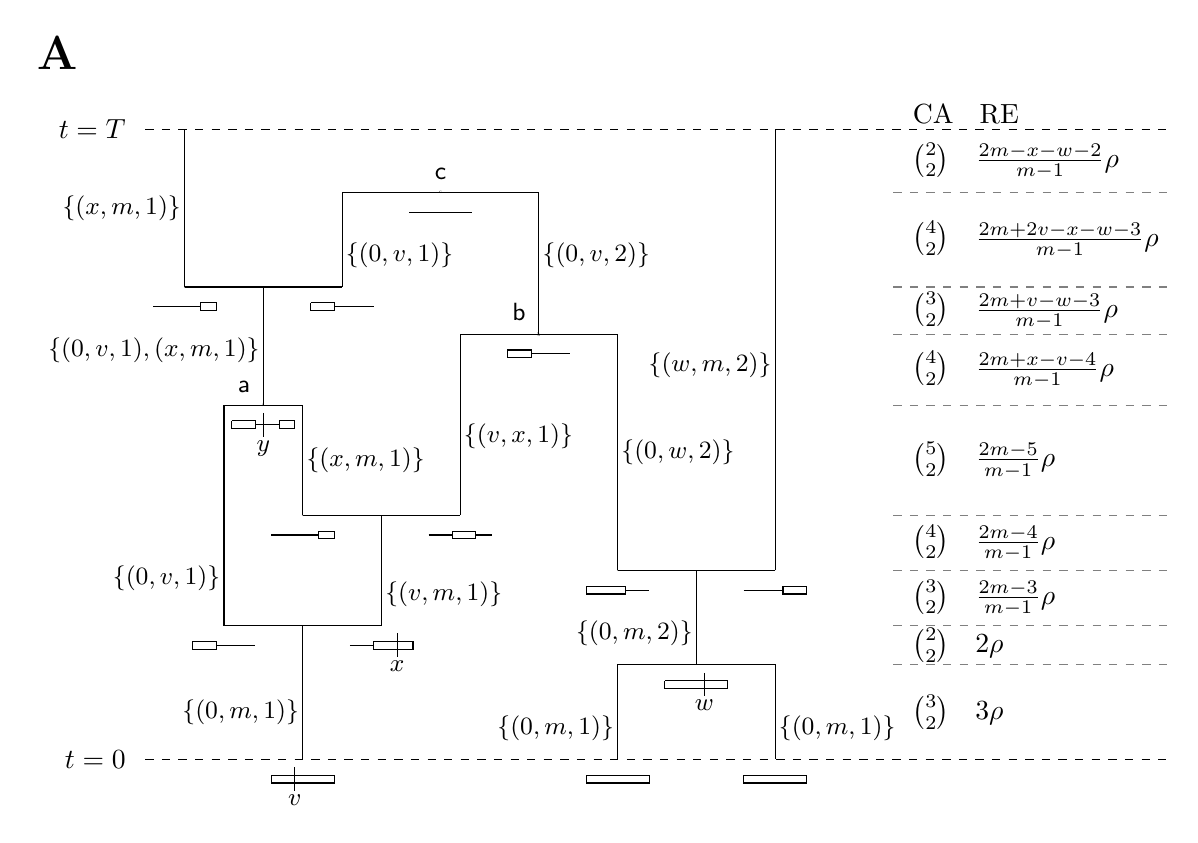
\begin{tikzpicture}
	\node [anchor=north west] at (-3.5,9.3) {\LARGE \textbf{A}};
	\draw (-0.4, -0.2) -- (0.4, -0.2) -- (0.4, -0.3) -- (-0.4, -0.3) -- (-0.4, -0.2);
	\draw (-0.1, -0.1) -- (-0.1, -0.4);
	\node [label=below:{\small $v$}] at (-0.1, -0.2) {};
	\draw (3.6, -0.2) -- (4.4, -0.2) -- (4.4, -0.3) -- (3.6, -0.3) -- (3.6, -0.2);
	\draw (5.6, -0.2) -- (6.4, -0.2) -- (6.4, -0.3) -- (5.6, -0.3) -- (5.6, -0.2);

	\draw (4,0) -- (4, 1.2) -- (6, 1.2) -- (6,0);
	\draw (4.6, 1) -- (5.4, 1) -- (5.4, 0.9) -- (4.6, 0.9) -- (4.6, 1);
	\draw (5.1, 1.1) -- (5.1, 0.8);
	\node [label=below:{\small $w$}] at (5.1, 1) {};

	\draw (0, 0) -- (0, 1.7) -- (-1,1.7) -- (1,1.7);
	\draw (-1.4, 1.5) -- (-1.1, 1.5) -- (-1.1, 1.4) -- (-1.4, 1.4) -- (-1.4, 1.5);
	\draw (-1.1, 1.45) -- (-0.6, 1.45);
	\draw (0.6, 1.45) -- (0.9, 1.45);
	\draw (0.9, 1.5) -- (1.4, 1.5) -- (1.4, 1.4) -- (0.9, 1.4) -- (0.9, 1.5);
	\draw (1.2, 1.6) -- (1.2, 1.3);
	\node [label=below:{\small $x$}] at (1.2, 1.5) {};

	\draw (5, 1.2) -- (5, 2.4) -- (4,2.4) -- (6,2.4);
	\draw (3.6, 2.2) -- (4.1, 2.2) -- (4.1, 2.1) -- (3.6, 2.1) -- (3.6, 2.2);
	\draw (4.1, 2.15) -- (4.4, 2.15);
	\draw (5.6, 2.15) -- (6.1, 2.15);
	\draw (6.1, 2.2) -- (6.4, 2.2) -- (6.4, 2.1) -- (6.1, 2.1) -- (6.1, 2.2);

	\draw (1, 1.7) -- (1, 3.1) -- (0,3.1) -- (2,3.1);
	\draw (-0.4, 2.85) -- (0.2, 2.85);
	\draw (0.2, 2.9) -- (0.4, 2.9) -- (0.4, 2.8) -- (0.2, 2.8) -- (0.2, 2.9);
	\draw (1.6, 2.85) -- (1.9, 2.85);
	\draw (1.9, 2.9) -- (2.2, 2.9) -- (2.2, 2.8) -- (1.9, 2.8) -- (1.9, 2.9);
	\draw (2.2, 2.85) -- (2.4, 2.85);

	\draw (-1, 1.7) -- (-1, 4.5) -- (0,4.5) -- (0,3.1);
	\node [scale=0.2,label=above left:{\small \textsf{a}}] at (-0.5,4.5) {a};
	\draw (-0.9, 4.3) -- (-0.6, 4.3) -- (-0.6, 4.2) -- (-0.9, 4.2) -- (-0.9, 4.3);
	\draw (-0.6, 4.25) -- (-0.3, 4.25);
	\draw (-0.3, 4.3) -- (-0.1, 4.3) -- (-0.1, 4.2) -- (-0.3, 4.2) -- (-0.3, 4.3);
	\draw (-0.5, 4.4) -- (-0.5, 4.1);
	\node [label=below:{\small $y$}] at (-0.5, 4.3) {};

	\draw (4,2.4) -- (4,5.4) -- (2,5.4) -- (2,3.1);
	\node [scale=0.2,label=above left:{\small \textsf{b}}] at (3,5.4) {b};
	\draw (2.6, 5.2) -- (2.9, 5.2) -- (2.9, 5.1) -- (2.6, 5.1) -- (2.6, 5.2);
	\draw (2.9, 5.15) -- (3.4, 5.15);

	\draw (-0.5, 4.5) -- (-0.5, 6) -- (-1.5,6) -- (0.5,6);
	\draw (-1.9, 5.75) -- (-1.3, 5.75);
	\draw (-1.3, 5.8) -- (-1.1, 5.8) -- (-1.1, 5.7) -- (-1.3, 5.7) -- (-1.3, 5.8);
	\draw (0.1, 5.8) -- (0.4, 5.8) -- (0.4, 5.7) -- (0.1, 5.7) -- (0.1, 5.8);
	\draw (0.4, 5.75) -- (0.9, 5.75);

	\draw (0.5, 6) -- (0.5, 7.2) -- (3,7.2) -- (3,5.4);
	\node [scale=0.2,label=above:{\small \textsf{c}}] at (1.75,7.2) {c};
	\draw (1.35, 6.95) -- (2.15, 6.95);

	\draw (-1.5, 6) -- (-1.5, 8);
	\draw (6, 2.4) -- (6, 8);

	% Edge annotations above each event
	\node [label=left:{\small$\{(0,m,1)\}$}] at (0.2,0.6) {};
	\node [label=left:{\small$\{(0,m,1)\}$}] at (4.2,0.4) {};
	\node [label=right:{\small$\{(0,m,1)\}$}] at (5.8,0.4) {};
	\node [label=left:{\small$\{(0,m,2)\}$}] at (5.2,1.6) {};
	\node [label=left:{\small$\{(0,v,1)\}$}] at (-0.8,2.3) {};
	\node [label=right:{\small$\{(v,m,1)\}$}] at (0.8,2.1) {};
	\node [label=right:{\small$\{(0,w,2)\}$}] at (3.8,3.9) {};
	\node [label=left:{\small$\{(w,m,2)\}$}] at (6.2,5) {};
	\node [label=right:{\small$\{(x,m,1)\}$}] at (-0.2,3.8) {};
	\node [label=right:{\small$\{(v,x,1)\}$}] at (1.8,4.1) {};
	\node [label=left:{\small$\{(0,v,1), (x,m,1)\}$}] at (-0.3,5.2) {};
	\node [label=right:{\small$\{(0,v,2)\}$}] at (2.8,6.4) {};
	\node [label=left:{\small$\{(x,m,1)\}$}] at (-1.3,7) {};
	\node [label=right:{\small$\{(0,v,1)\}$}] at (0.3,6.4) {};

	% Dashed lines for start and end times
	\draw[dashed] (-2, 0) -- (11, 0);
	\node [label=left:{$t = 0$}] at (-2,0) {};
	\draw[dashed] (-2, 8) -- (11, 8);
	\node [label=left:{$t = T$}] at (-2,8) {};

	% Numbers of extant ancestors and links, from top to bottom
	\node[label=right:{CA \; RE}] at (7.5, 8.2) {};
	\node[label=right:{$\binom{2}{2}$ \; $\frac{2 m - x - w - 2}{m - 1} \rho$}] at (7.5, 7.6) {};
	\node[label=right:{$\binom{4}{2}$ \; $\frac{2 m + 2 v - x - w - 3}{m - 1} \rho$}] at (7.5, 6.6) {};
	\node[label=right:{$\binom{3}{2}$ \; $\frac{2 m + v - w - 3}{m - 1} \rho$}] at (7.5, 5.7) {};
	\node[label=right:{$\binom{4}{2}$ \; $\frac{2 m + x - v - 4}{m - 1} \rho$}] at (7.5, 4.95) {};
	\node[label=right:{$\binom{5}{2}$ \; $\frac{2 m - 5}{m - 1} \rho$}] at (7.5, 3.8) {};
	\node[label=right:{$\binom{4}{2}$ \; $\frac{2 m - 4}{m -1} \rho$}] at (7.5, 2.75) {};
	\node[label=right:{$\binom{3}{2}$ \; $\frac{2 m - 3}{m - 1} \rho$}] at (7.5, 2.05) {};
	\node[label=right:{$\binom{2}{2}$ \; $2 \rho$}] at (7.5, 1.45) {};
	\node[label=right:{$\binom{3}{2}$ \; $3 \rho$}] at (7.5, 0.6) {};

	% Gray dashed lines to visually separate holding times
	\draw[color=gray, dashed] (7.5, 1.2) -- (11, 1.2);
	\draw[color=gray, dashed] (7.5, 1.7) -- (11, 1.7);
	\draw[color=gray, dashed] (7.5, 2.4) -- (11, 2.4);
	\draw[color=gray, dashed] (7.5, 3.1) -- (11, 3.1);
	\draw[color=gray, dashed] (7.5, 4.5) -- (11, 4.5);
	\draw[color=gray, dashed] (7.5, 5.4) -- (11, 5.4);
	\draw[color=gray, dashed] (7.5, 6) -- (11, 6);
	\draw[color=gray, dashed] (7.5, 7.2) -- (11, 7.2);
\end{tikzpicture}
&
\begin{tikzpicture}
	\node [anchor=north west] at (-3.5,9.3) {\LARGE \textbf{B}};
	\draw (-0.4, -0.2) -- (0.4, -0.2) -- (0.4, -0.3) -- (-0.4, -0.3) -- (-0.4, -0.2);
	\draw (-0.1, -0.1) -- (-0.1, -0.4);
	\node [label=below:{\small $v$}] at (-0.1, -0.2) {};
	\draw (3.6, -0.2) -- (4.4, -0.2) -- (4.4, -0.3) -- (3.6, -0.3) -- (3.6, -0.2);
	\draw (5.6, -0.2) -- (6.4, -0.2) -- (6.4, -0.3) -- (5.6, -0.3) -- (5.6, -0.2);

	\draw (4,0) -- (4, 1.2) -- (6, 1.2) -- (6,0);
	\draw (4.6, 1) -- (5.4, 1) -- (5.4, 0.9) -- (4.6, 0.9) -- (4.6, 1);
	\draw (5.1, 1.1) -- (5.1, 0.8);
	\node [label=below:{\small $w$}] at (5.1, 1) {};

	\draw (0, 0) -- (0, 1.7) -- (-1,1.7) -- (1,1.7);
	\draw (-1.4, 1.5) -- (-1.1, 1.5) -- (-1.1, 1.4) -- (-1.4, 1.4) -- (-1.4, 1.5);
	\draw (-1.1, 1.45) -- (-0.6, 1.45);
	\draw (0.6, 1.45) -- (0.9, 1.45);
	\draw (0.9, 1.5) -- (1.4, 1.5) -- (1.4, 1.4) -- (0.9, 1.4) -- (0.9, 1.5);
	\draw (1.2, 1.6) -- (1.2, 1.3);
	\node [label=below:{\small $x$}] at (1.2, 1.5) {};

	\draw (5, 1.2) -- (5, 2.4) -- (4,2.4) -- (6,2.4);
	\draw (3.6, 2.2) -- (4.1, 2.2) -- (4.1, 2.1) -- (3.6, 2.1) -- (3.6, 2.2);
	\draw (4.1, 2.15) -- (4.4, 2.15);
	\draw (5.6, 2.15) -- (6.1, 2.15);
	\draw (6.1, 2.2) -- (6.4, 2.2) -- (6.4, 2.1) -- (6.1, 2.1) -- (6.1, 2.2);
	\draw [color=red](5.8, 2.3) -- (5.8, 2.0);
	\node [label={[red]below:{\small $z$}}] at (5.8, 2.1) {};

	\draw (1, 1.7) -- (1, 3.1) -- (0,3.1) -- (2,3.1);
	\draw (-0.4, 2.85) -- (0.2, 2.85);
	\draw (0.2, 2.9) -- (0.4, 2.9) -- (0.4, 2.8) -- (0.2, 2.8) -- (0.2, 2.9);
	\draw (1.6, 2.85) -- (1.9, 2.85);
	\draw (1.9, 2.9) -- (2.2, 2.9) -- (2.2, 2.8) -- (1.9, 2.8) -- (1.9, 2.9);
	\draw (2.2, 2.85) -- (2.4, 2.85);

	\draw (-1, 1.7) -- (-1, 4.5) -- (0,4.5) -- (0,3.1);
	\draw (-0.9, 4.3) -- (-0.6, 4.3) -- (-0.6, 4.2) -- (-0.9, 4.2) -- (-0.9, 4.3);
	\draw (-0.6, 4.25) -- (-0.3, 4.25);
	\draw (-0.3, 4.3) -- (-0.1, 4.3) -- (-0.1, 4.2) -- (-0.3, 4.2) -- (-0.3, 4.3);
	\draw (-0.5, 4.4) -- (-0.5, 4.1);
	\node [label=below:{\small $y$}] at (-0.5, 4.3) {};

	\draw (6, 2.4) -- (6, 3.8) -- (7, 3.8);
	\draw [color=red](6, 3.8) -- (5, 3.8);
	\draw (4.6, 3.55) -- (5.4, 3.55);
	\draw (6.6, 3.55) -- (7.1, 3.55);
	\draw (7.1, 3.6) -- (7.4, 3.6) -- (7.4, 3.5) -- (7.1, 3.5) -- (7.1, 3.6);

	\draw (4,2.4) -- (4,5.4) -- (2,5.4) -- (2,3.1);
	\draw (2.6, 5.2) -- (2.9, 5.2) -- (2.9, 5.1) -- (2.6, 5.1) -- (2.6, 5.2);
	\draw (2.9, 5.15) -- (3.4, 5.15);

	\draw (-0.5, 4.5) -- (-0.5, 6) -- (-1.5,6) -- (0.5,6);
	\draw (-1.9, 5.75) -- (-1.3, 5.75);
	\draw (-1.3, 5.8) -- (-1.1, 5.8) -- (-1.1, 5.7) -- (-1.3, 5.7) -- (-1.3, 5.8);
	\draw (0.1, 5.8) -- (0.4, 5.8) -- (0.4, 5.7) -- (0.1, 5.7) -- (0.1, 5.8);
	\draw (0.4, 5.75) -- (0.9, 5.75);

	\draw [color=red](5, 3.8) -- (5, 6.6) -- (4, 6.6);
	\draw (4,6.6) -- (3,6.6) -- (3, 5.4);
	\draw (3.6, 6.4) -- (3.9, 6.4) -- (3.9, 6.3) -- (3.6, 6.3) -- (3.6, 6.4);
	\draw (3.9, 6.35) -- (4.4, 6.35);

	\draw (0.5, 6) -- (0.5, 7.2) -- (4,7.2) -- (4,6.6);
	\draw (1.85, 6.95) -- (2.65, 6.95);

	\draw (-1.5, 6) -- (-1.5, 8);
	\draw [color=red](2.25, 7.2) -- (2.25, 8);
	\draw (7, 3.8) -- (7, 8);

	% Dashed lines for start and end times
	\draw[dashed] (-2, 0) -- (9.1, 0);
	\node [label=left:{$t = 0$}] at (-2,0) {};
	\draw[dashed] (-2, 8) -- (9.1, 8);
	\node [label=left:{$t = T$}] at (-2,8) {};

	% Numbers of extant ancestors and links, from top to bottom
	\node[label=right:{CA \; RE}] at (7.5, 8.2) {};
	\node[label=right:{$\binom{3}{2}$ \; $3 \rho$}] at (7.5, 7.6) {};
	\node[label=right:{$\binom{4}{2}$ \; $4 \rho$}] at (7.5, 6.9) {};
	\node[label=right:{$\binom{5}{2}$ \; $5 \rho$}] at (7.5, 6.3) {};
	\node[label=right:{$\binom{4}{2}$ \; $4 \rho$}] at (7.5, 5.7) {};
	\node[label=right:{$\binom{5}{2}$ \; $5 \rho$}] at (7.5, 4.95) {};
	\node[label=right:{$\binom{6}{2}$ \; $6 \rho$}] at (7.5, 4.15) {};
	\node[label=right:{$\binom{5}{2}$ \; $5 \rho$}] at (7.5, 3.45) {};
	\node[label=right:{$\binom{4}{2}$ \; $4 \rho$}] at (7.5, 2.75) {};
	\node[label=right:{$\binom{3}{2}$ \; $3 \rho$}] at (7.5, 2.05) {};
	\node[label=right:{$\binom{2}{2}$ \; $2 \rho$}] at (7.5, 1.45) {};
	\node[label=right:{$\binom{3}{2}$ \; $3 \rho$}] at (7.5, 0.6) {};

	% Gray dashed lines to visually separate holding times
	\draw[color=gray, dashed] (7.5, 1.2) -- (9.1, 1.2);
	\draw[color=gray, dashed] (7.5, 1.7) -- (9.1, 1.7);
	\draw[color=gray, dashed] (7.5, 2.4) -- (9.1, 2.4);
	\draw[color=gray, dashed] (7.5, 3.1) -- (9.1, 3.1);
	\draw[color=gray, dashed] (7.5, 3.8) -- (9.1, 3.8);
	\draw[color=gray, dashed] (7.5, 4.5) -- (9.1, 4.5);
	\draw[color=gray, dashed] (7.5, 5.4) -- (9.1, 5.4);
	\draw[color=gray, dashed] (7.5, 6) -- (9.1, 6);
	\draw[color=gray, dashed] (7.5, 6.6) -- (9.1, 6.6);
	\draw[color=gray, dashed] (7.5, 7.2) -- (9.1, 7.2);
\end{tikzpicture}
\end{tabular}
}
\caption{(A)
A realisation of the graph traversed by Hudson's algorithm started from a
sample of three chromosomes of length $m$ at time $t = 0$, and
propagated until time $T$. The MRCA on the genetic interval $[v, w)$ is reached
at event \textsf{b}, while that on $[0, v)$ is reached at event \textsf{c}.
The non-ancestral segment $[v, w)$ above
A contributes to the rate of effective recombinations because it
is trapped between ancestral segments. The two columns titled CA and RE
are the respective rates of mergers and recombinations when
the recombination rate is $\rho$.
(B) A corresponding realisation of a big ARG, which augments Hudson's algorithm
by tracking nonancestral lineages. The result is a simpler state space and
dynamics, at the cost of extra nodes and edges, highlighted in red, which do
not affect the local tree at any site.}
\label{hudson_vs_bigARG}
\end{figure}

% Full quote:
% This process simplifies mathematics on the account that the notion of an
% ancestor will have a less restrictive meaning than usual:
% An ``ancestral'' sequence in the birth and death process
% need not have any genetic material in common with a
% sequence descended from it.

\subsection*{Survey of ARG inference methods}

The problem of reconstructing ARGs for samples of recombining sequences has
been of interest since the ARG was first defined. Early methods focused on
finding \emph{parsimonious} ARGs, i.e.\ those with a minimal number of
recombination events \citep{hein1990reconstructing}. Two main approaches
emerged: \emph{backwards-in-time} \citep{lyngso2005minimum} and
\emph{along-the-genome} \citep{song2003parsimonious, song2005constructing}. The
former starts with a data matrix and reduces it to an empty matrix through row
and column operations corresponding to coalescence, mutation, and recombination
events, which construct an ARG from the bottom up. The latter begins from an
initial local tree at a single focal site. Moving the focal site along the
genome changes the local tree via a \emph{subtree prune and regraft} (SPR)
operation whenever a recombination is encountered. Methods based the
backwards-in-time approach are described by \citet{song2005efficient,
wu2008association, thao2019hybrid, ignatieva2021kwarg}, while
\citet{hein1993heuristic, wu2011new, mirzaei2017rent} describe along-the-genome
methods. \citet{rasmussen2022espalier} focuses on parsimonious fusion of local
trees into an ARG, while \citet{camara2016inference} is based on topological
data analysis.

Reconstructing a most parsimonious ARG for a given data set is NP-hard
\citep{wang2001perfect}, so parsimony-based methods resort to heuristics and
are limited to analysing at most hundreds of sequences. Hence, a number of
methods aim to balance computational efficiency with reconstruction of
``reasonable", rather than parsimonious ARGs \citep{minichiello2006mapping,
parida2008estimating, kelleher2019inferring,  speidel2019method,
zhang2023biobank}. The latter three methods, as well as the parsimony-based
method of \citet{rasmussen2022espalier}, can be used on megabase scale data and
hundreds of thousands of samples under human-like parameters.

TODO mention \citep{schaefer2021ancestral} somewhere.
Also \citep{kuhner2017consensus}.

% AI: just to note, these papers do not all agree in their definition of an
% ARG. I guess this is one of the points of the present paper, but should we
% mention this fact? Should we also mention that most of these infer just the
% topology, but some also the times?

An alternative approach is to treat the ARG as a latent parameter to be
averaged out by Monte Carlo methods, based either on importance sampling
\citep{griffiths1996ancestral, fearnhead2001estimating, jenkins2011inference}
or MCMC \citep{kuhner2000maximum, nielsen2000estimation, wang2008bayesian,
fallon2013acg, mahmoudi2022bayesian}. These methods operate on representations
of the ``little ARG'', and are extremely computationally expensive, being
applicable to at most hundreds of samples consisting of tens or hundreds of
kilobases with human-like parameters. State-of-the-art methods rely on cheaper,
approximate models \citep{didelot2010inference, heine2018bridging,
hubisz2020mapping,hubisz2020inference, medina2020speeding}. The most scalable
method, \texttt{ARGWeaver} \citep{rasmussen2014genome}, can be applied to
dozens of mammal-like genomes \citep{hubisz2020inference}. A central quantity
in all of these sampling methods is the conditional sampling probability $p(G |
D) \propto p(D | G) p(G)$ of an ARG $G$ given an observed realization of
genetic diversity $D$ at its sampled leaves, where $p(D | G)$ is the likelihood
of the data $D$ given $G$, and $p(G)$ is a Bayesian prior distribution or a
frequentist regularizer for the ARG $G$.

The likelihood $p(D | G)$ is effectively always the distribution of a Poisson
process on the ancestral material along the edges of $G$ \citep[Eq.\
(2)]{mahmoudi2022bayesian}. Hence it is typically straightforward to evaluate
in principle, but choosing the right data structure can still have a dramatic
effect on the efficiency of evaluation \citep{mahmoudi2022bayesian}. Especially
in the Bayesian case, $p(G)$ is typically specified as the sampling
distribution of a stochastic process, such as the coalescent with
recombination. Two contemporary examples are \cite{mahmoudi2022bayesian,
guo2022recombination}. Evaluating the distribution of the coalescent with
recombination (or related models) requires knowledge of the number of extant
lineages and number of links available for recombination (i.e.\ ones at which a
recombination would split ancestral material) at each time \citep[Eq.\
(3)]{mahmoudi2022bayesian}. These require a data structure from which shared
edges on different trees are easy to identify, and which encodes recombination
events and times explicitly, e.g.\ using nodes.
We will provide a more detailed discussion on sampling probability evaluation in the appendix.
\end{document}
